% !TEX program = arara
% arara: pdflatex
% arara: biber
% arara: pdflatex
% arara: pdflatex
% arara: clean: { files: [ Bericht.out ] }
% arara: clean: { files: [ Bericht.aux, Bericht.bbl ] }
% arara: clean: { files: [ Bericht.bcf, Bericht.blg ] }
% arara: clean: { files: [ Bericht.log, Bericht.run.xml ] }
% arara: clean: { files: [ Bericht.toc, Bericht-blx.bib ] }
% 

\documentclass{Bericht}
\usepackage{todonotes}
\usepackage{float}

\begin{document}

\maketitle

% % % % %

\tableofcontents
\clearpage

\section{Einleitung}
\subsection{Einstieg}
\textit{Autor:} Kim\\
	Das Thema Zeitempfinden spielt in unserer modernisierten Gesellschaft eine immer wichtiger werdende Rolle, da es zwischen Arbeit, Freizeit und Familie wichtig ist seine Zeitgenau zu planen, um jede freie Minute ausnutzen zu können.	
	Aufgrund des Wissens, dass die arbeitende Bevölkerung sich an bestimmte Zeitregeln hält und versucht den Alltag optimal zu managen und unter Betrachtung der zunehmenden Relevanz von Zeitmanagement und dem Zeitsparen, richteten wir unsere Forschung auf das Thema der Zeitmanipulation. Zunächst gilt zu definieren, was Zeit überhaupt ist: "`Zeit ist das Nacheinander von Zuständen und Ereignissen, die erlebbar und messbar sind. Sie ist eine physikalische Größe für die Vergänglichkeit und Veränderungen“. \todo{zitat?}

	In unserer Lebenswelt gibt es bestimmte Zeitgeber, von der Uhrzeit selber einmal abgesehen, die uns Hinweise geben, wieviel Zeit vergangen ist. Für uns galt es nun herauszufinden, ob es möglich ist, anhand gängiger Zeitgeber, die jeden einzelnen Menschen seit der Geburt täglich begleiten, eine Manipulation des Zeitempfindens auszulösen. Anhand unserer Forschungsfrage: ,,Wie stark lässt sich das menschliche
Zeitempfinden durch in der VR eingesetzte visuelle und auditive Zeitgeber manipulieren und
wie nachhaltig ist der Einfluss eines Aufenthalts in der VR auf das menschliche Zeitempfinden
im realen Leben?'' erschufen wir eine Virtuelle Welt, durch die unsere späteren Versuchspersonen mit Hilfe einer VR-Brille manipulierte Zeitgeber erlebten. 

	 Wir legten einen weiteren Fokus unserer Arbeit auf die Zeitschätzung. Jede Versuchsperson wurde gebeten, vor und nach dem Befinden in der virtuellen Welt eine bestimmte Sekundenanzahl abzuschätzen, ohne auf Hilfsmittel zuzugreifen, wie beispielsweise eine Armbanduhr. Auf diese Weise wollten wir herausfinden, ob sich die Zeitschätzung vor dem Befinden in der Virtuellen Welt von der Zeitschätzung nach dem Befinden in der Virtuellen Welt unterscheidet.
Dieser Bericht führt über die Ideenfindung unserer Forschungsschwerpunktes zu unseren Hypothesen. Nach der technischen und kreativen Umsetzung unseres Experiments und unserer virtuellen Welt wird der detaillierte Ablauf des Experiments beschrieben. Im Zweiten Teil- dem empirischen Teil- folgen die Auswertungen, Ergebnisse und Interpretationen und der Bezug zu unseren Hypothesen. Am Ende des Berichts gibt es einen kurzen Überblick über die Zusammenarbeit der Forschungsgruppe und ein abschließendes Fazit. 

	Ob  Albert Einsteins Definition von Zeit \textit{"`Zeit ist das, was man an der Uhr abliest.'' } wirklich ausreicht, oder ob es andere wichtige Zeitgeber gibt, die das menschliche Zeitempfinden vorgeben, gilt es herauszufinden. 

\label{subsec:ideenfindung}
\subsection{Ideenfindung und Fragestellung}
\textit{Autor:} Berna, \textit{Überarbeitung:} Jana\\
Zu Beginn des Projekts wurden mithilfe der Brainstorming-Methode erste Ideen gesammelt, um eine grobe Vorstellung zu bekommen, wie sich das Experiment aufbauen lässt. Dabei wurden überzogene und -schwer realisierbare Vorstellungen nicht sofort verworfen und ein kreatives Denken ermutigt.
Ersten Ideen gingen in Richtung Phobiebewältigung (bspw. Spinnen oder Höhe) und allgemeine Body-Ownership-Konzepte (z.B. die Versuchsperson in einen Körper des anderen Geschlechts oder Hautfarbe zu versetzen und festzustellen, ob sie diesen als ihren eigenen wahrnehmen kann). Weiterhin wurden auch schwieriger umsetzbare Konzepte geäußert, wie das Steuern eines Rollstuhls durch Gedanken und moralisch anspruchsvolle Themen wie die Frage, wie weit Versuchspersonen in der VR gehen, wenn sie zum Töten aufgefordert werden.\\
Im weiteren Verlauf wurde recherchiert, ob bereits Experimente in diese Richtungen geführt wurden und in der Gruppe diskutiert, wie sich auf diese aufbauen ließe. Parallel wurden auch weiterhin neue Ideen in Betracht gezogen und diskutiert. Besonderes Interesse fand die in dieser Phase die Frage, inwieweit die VR einen Einfluss auf Reaktionsfähigkeit oder Bewegungsablauf eines Menschen hat. Auf dieser Grundlage sollten innerhalb der VR Reaktionstests durchgeführt werden, wie bspw. das Fangen von Gegenständen. Um ein vollständiges Immersionserlebnis zu gewährleisten wären hier die Implemenation von Hand-Trackern und möglicherweise auch Spiegelugen der Versuchsperson nötig (,,body transfer illusion''). Die Grundlagenforschung zur Zeitwahrnehmung in der VR von Gerd Bruder gab den Anlass, den Forschungsschwerpunkt auf Zeitwahrnehmung und -manipulation zu verlagern. Darauf aufbauend wurde die erste Forschungsfrage formuliert:
\textit{,,Wie verändert sich das Zeitempfinden in der realen Welt auf den Avatar durch einwirkende Zeitraffung bzw. Zeitdehnung in der Virtual Reality?''}\\
	 Der Fokus liegt hier bereits auf dem subjektiven Zeitempfinden der Versuchsperson. Der Aufbau der virtuellen Testumgebung sollte alltäglichen Situationen nachempfunden sein und zu neben Zeitmanipulatoren (z.B. Geschwindigkeit von Autos, Wolken und Gravitation) im direkten Umfeld auch Aufgaben beinhalten, die die Versuchsperson zu erfüllen hat. Schnelle, langsame und normale Zeitgeber sollten auf drei unterschiedliche Karten verteilt werden und jeweils ein Drittel der Versuchspersonen eine dieser Testumgebungen durchlaufen. Hierbei sollte herausgefunden werden, wie sich die Zeitwahrnehmung durch die verschiedenen Zeitgeber verändert und ob es Unterschiede in den Testumgebungen gibt. Aufgrund der Studie ,,Could Virtual Reality Help Manipulate Time Perception?'' einer Forschungsgruppe der Universität Hamburg (vgl. Kapitel 1.3 im Paper) wurde das Experimentdesign umstrukturiert und die internen Aufgaben weggelassen.\\
Ebenfalls wurde das Experimentdesign nach einiger Überlegung und Rücksprachen als zu umfangreich bewertet, sodass die drei Karten auf eine reduziert wurden, in welcher sich bereits alle Zeitgeber befinden und die die Versuchsperson während ihres Aufenthalts ohne große Ablenkungen auf sich wirken lassen kann. Als besonderen Aspekt wurden visuelle und akustische Zeitgeber gesondert betrachtet, wobei von jedem dieser je ein schneller und ein langsamer verwendet wird. Der zweite gewählte Fokus der Arbeit liegt weiterhin auf dem Einfluss der VR auf auf die Realität.  
Das Experiment wurde also deutlich verkürzt und die Fragestellung angepasst: \textit{,,Wie stark lässt sich das menschliche
Zeitempfinden durch in der VR eingesetzte visuelle und auditive Zeitgeber manipulieren und
wie nachhaltig ist der Einfluss eines Aufenthalts in der VR auf das menschliche Zeitempfinden
im realen Leben?''} 
 
\subsection{Planung}

 % Marvin
		%Erster Kontakt
		Erster Berührungspunkt mit dem Bachelorprojekt ¡Experiment! war für die Gruppenmitglieder die Vorstellung durch Thorsten Kluß am 24.01.2017 an der Hochschule für Künste, bzw. dessen Wiederholung am 06.04.2017 an der Universität Bremen. Erweitert wurde der zweite Termin dabei durch eine Führung durch das Cartesiums Bremen, sowie einer Beschreibung der vorangegangen Bachelorprojekte. Hierdurch konnte ein erster Eindruck über die verschiedenen Versuchsaufbauten und ferner der Möglichkeiten unseres Projekts gewonnen werden.\\
Die Gruppenmitglieder erstellten persönliche ,,Skill-Profile'', welche die eigenen Stärken und Schwächen darlegten und anhand derer sich die Gruppenmitglieder in zwei Teams einteilen ließen: das Technikteam (bestehend aus Marvin Becker, Nicole Dörnbach, Alina Escher, Jovana Kaurin, Svenja Kettenburg, Daniel Schmidt und Jana Wahls), welches primär für die Erstellung der virtuellen Testumgebung verantwortlich war und das Organisationsteam (bestehend aus Nizan Averbuh, Kim Brüning und Berna Sen), welche sich um das Anwerben von Versuchspersonen, die Beschaffung benötigter Dokumente und andere organisatorische Dinge kümmerte.
Darüber hinaus wurde entschieden, das Scrum-Modell projektbegleitend zu verwenden.\\
Es wurden vier Termine in der Woche ermittelt, welche für Gruppen- oder Teamtreffen genutzt werden können und mit einem zusätzlichen Zeitfenster am Donnerstag für ein Treffen mit den Dozenten. Ferner wurde für die Protokollführung der Treffen eine feste Reihenfolge angelegt.\\
Treffen fanden je nach Situation im Konferenzraum 4.43 des vierten Stockwerks oder den Räumen 4.12 und 4.16 (ebenfalls vierter Stock) im Cartesium statt, da kein für das Projekt dedizierter Raum dauerhaft unbesetzt war. Um Zugang zu der Etage und diesen Räumen zu gewährleisten, erhielten wir Türchips.\\
Auch wurden alle technischen Lösungen zur Arbeitsweise innerhalb der ersten zwei Wochen implementiert. Als zentrale Sammelstelle für Dokumente und projektrelevante Informationen wurde ein Board beim Service "`Trello'' genutzt. Dort wurden wöchentlichen Sprints sowie der Scrum-Backlog, die Protokolle oder die Termine der Treffen abgelegt. Für schnelle Kommunikation untereinander wurde der Nachrichtendienst "`WhatsApp'' genutzt, die Kommunikation zu den Dozenten lief per Email und in dringenden Fällen Telefonaten.\\
		Die genauen Spezifikationen an unser Experiment gemäß der Forschungsfrage wurden nach Rücksprache mit den Dozenten immer wieder verändert. Hierdurch entstand viel unbenutztes Material, da wir parallel bereits damit begonnen hatten, 3D-Objekte nach den ersten Anforderungen für unsere Versuchswelt zu erstellen. Dies geschah fälschlicherweise aus dem Versuch heraus, bereits verlorene Zeit aufzuholen, wodurch jedoch nur weiterer Verschnitt produziert worden ist, was uns umso mehr Zeit gekostet hat.\\
		Wir approximierten, dass sich ab diesem Zeitpunkt unser Projekt in 3 Phasen (Programmierphase, Versuchsphase, Evaluation/Paper) unterteilen ließe und legten Fristen für die einzelnen fest. Im Laufe des Projektes sollten wir jedoch erkennen, wie weit diese Einschätzungen von der Realität abwichen.Zu Beginn eines jeden Arbeitstages wurde ein 10-minütiges "`Scrum-Treffen'' abgehalten, in dem anstehende Aufgaben aus dem Backlog und Probleme besprochen wurden. Diese Treffen wurden jedoch insbesondere in späteren, arbeitsintensiveren Phasen vernachlässigt.\\

		
		\begin{figure}[H] % here - top - bottom - page, das ! erzwingt die Position falls möglich
			\centering
			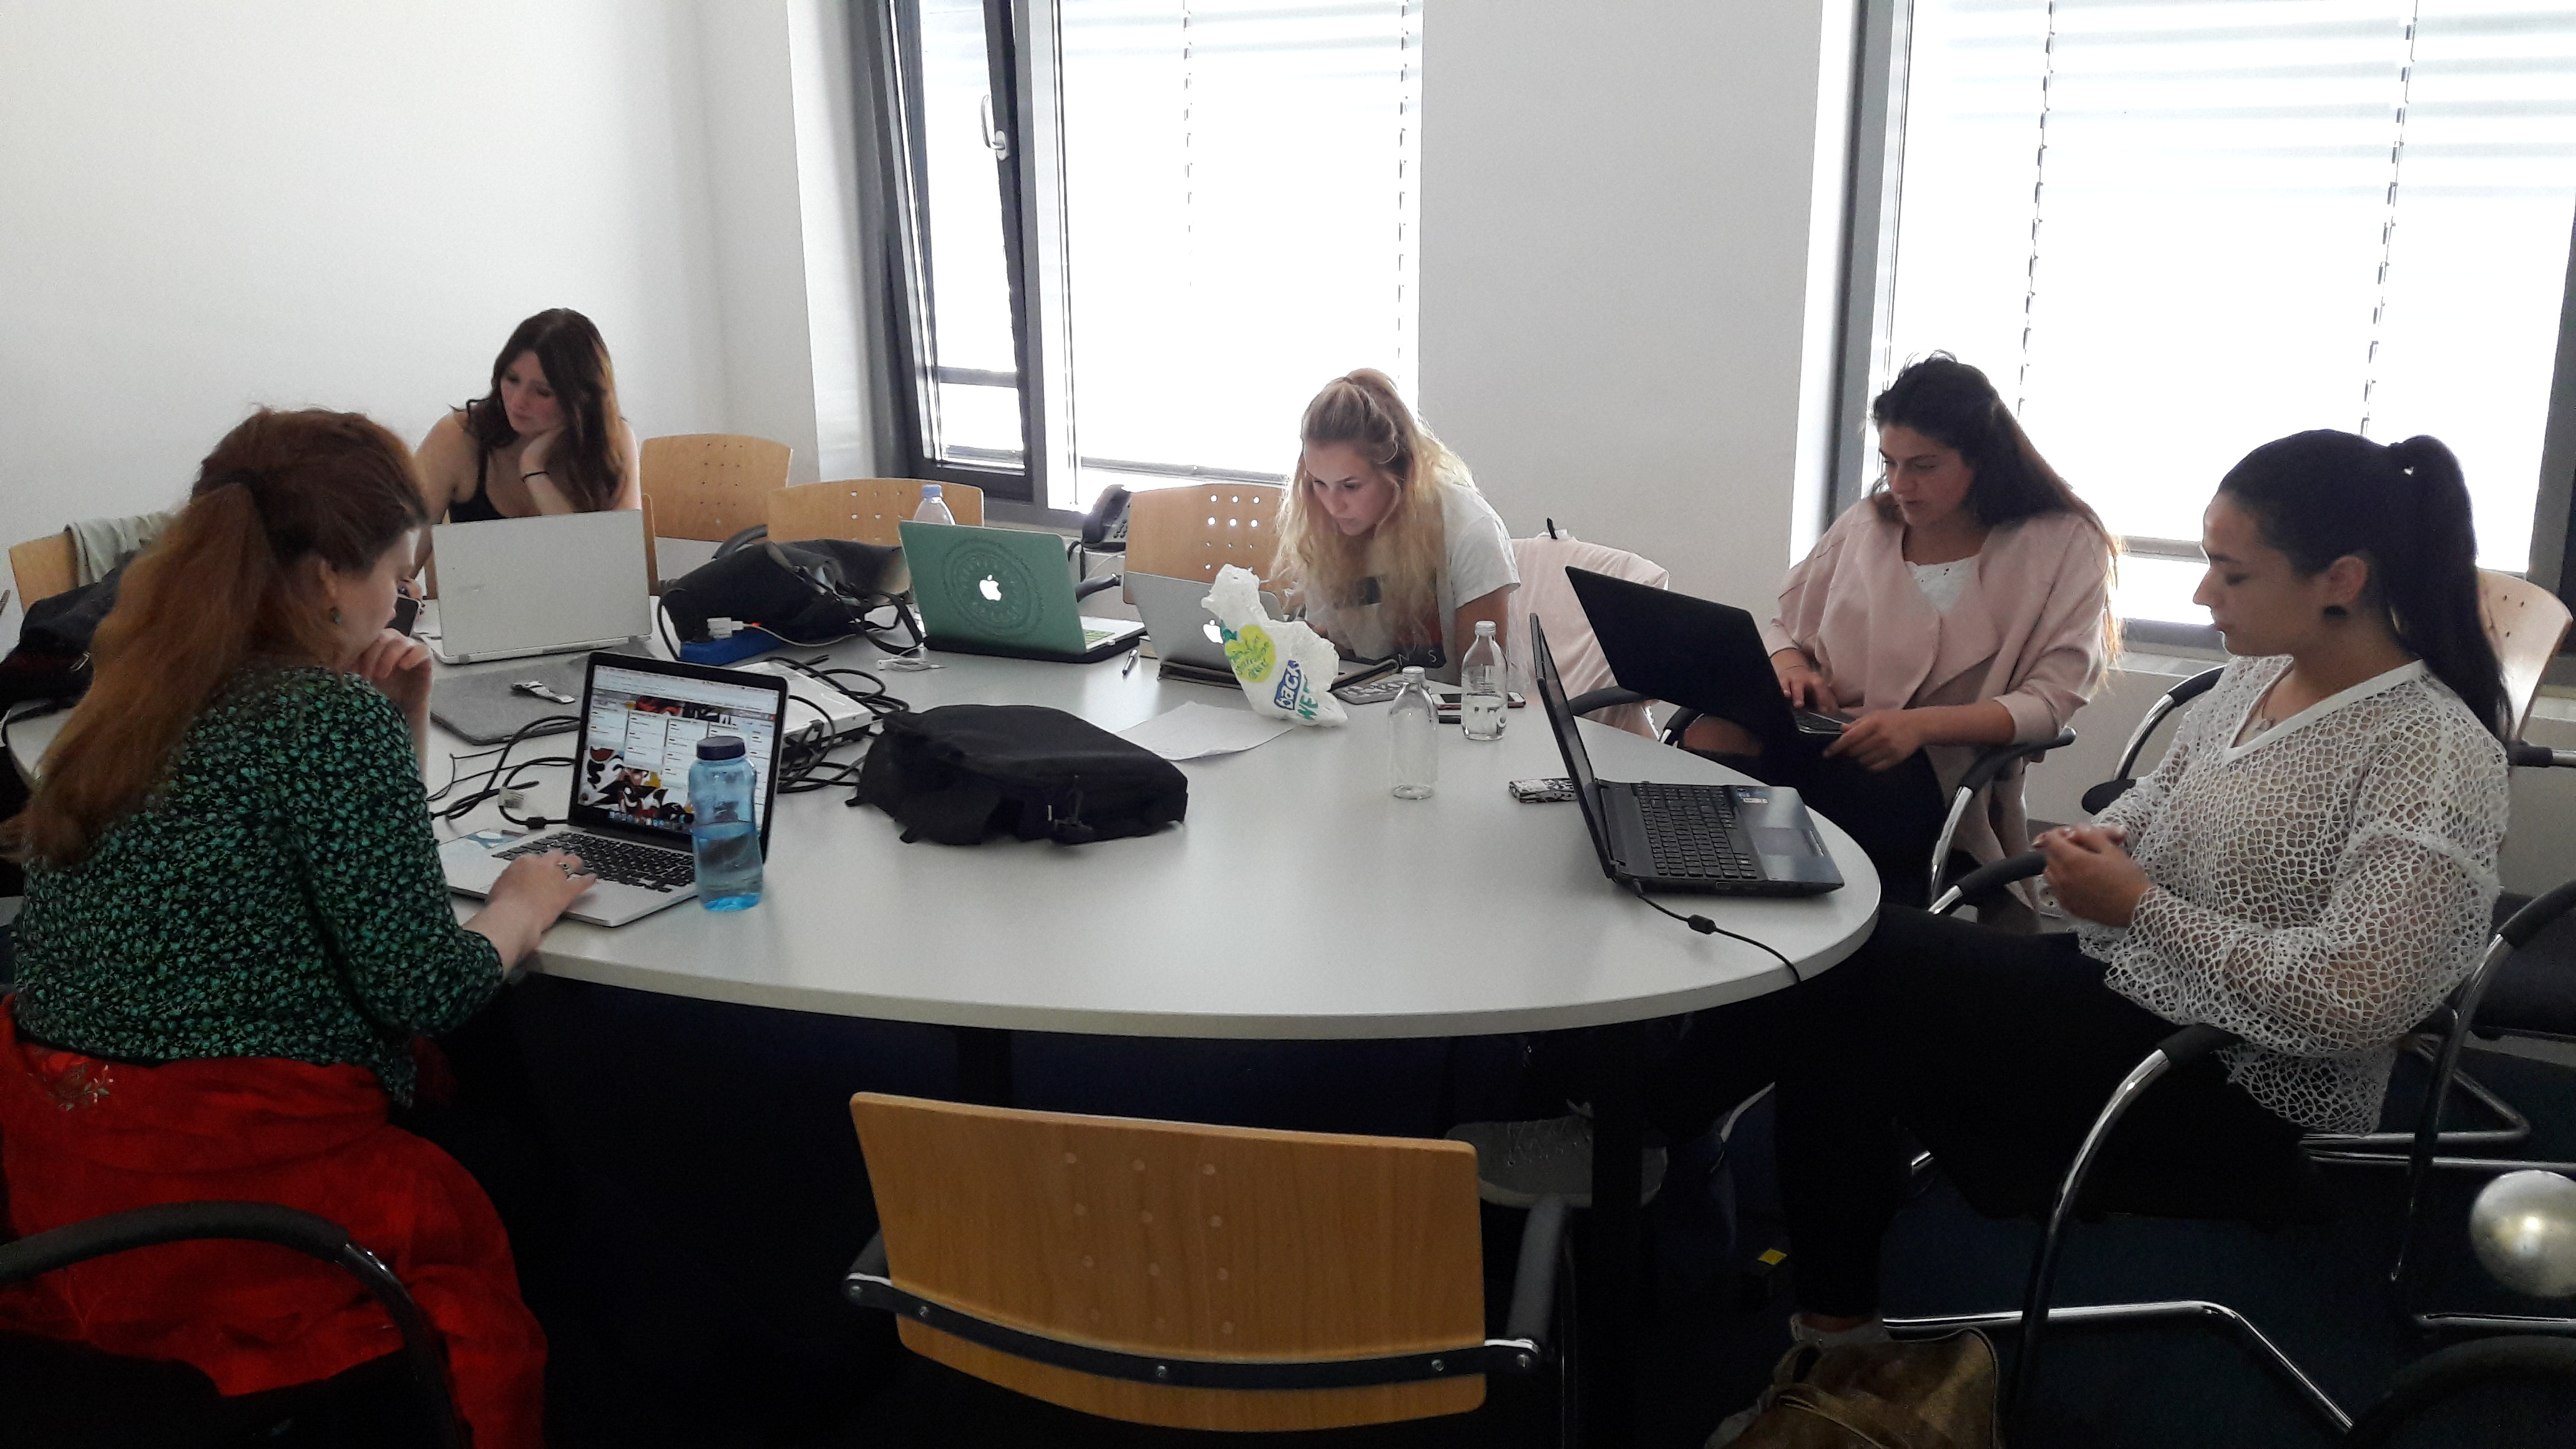
\includegraphics[width=\linewidth, height=\textheight, keepaspectratio]{../Bilder/20170518_103125.jpg}
			\caption{Das ¡Experiment!-Team bei der Arbeit}
			\label{img:experiment-team-bei-der-arbeit}
		\end{figure}
		


\section{Virtuelle Testumgebung}

\subsection{Experimentdesign}

Das Experimentdesign besteht einerseits aus der Gestaltung der virtuellen Testumgebung, deren Steuerung durch die Versuchsperson und der Erstellung begleitender Dokumente und Tests, um die Effekte nachweisen zu können.\\
Die Testumgebung wurde zunächst als Open-World-Konzept geplant, in welcher sich die Versuchsperson nach Belieben umsehen konnte. Dieses Konzept wurde verworfen, da Versuchspersonen auf diese Weise nicht das exakt gleiche erleben und Ergebnisse in dieser Hinsicht weniger aussagekräftig sind. Um die gleichen Eindrücke für jede Versuchspersonen zu gewährleisten, war das Implementieren einer vorgegebenen Route innerhalb der Testumgebung Voraussetzung (vgl. Kapitel \ref{subsec:aufbau}).
	Obwohl das Experimentdesign vorsah, die Navigation innerhalb der Testumgebung in der Virtusphere stattfinden zu lassen um das Immersionserlebnis zu erhöhen, musste aufgrund von erheblichen technischen Problemen diesbezüglich auf herkömmliche Controller ausgewichen werden.\\
	Die ermittelte Fragestellung und Hypothesen \textbf{noch nicht genannt} sollten empirisch überprüft werden, wobei genug Versuchspersonen am Experiment teilnehmen mussten.
Auf Grundlage der Rechercheergebnissen zur  Zeitmanipulation wurden die verwendeten Dokumente gestaltet. Hierbei wurden neben mehreren Fragebögen, welche Einflussfaktoren und Effekte der VR abfragen		 (vgl. Kapitel \ref{subsec:dokumente}) auch insgesamt sechs Zeiteinschätzungstests in den Ablauf integriert, welche den allgemeinen Einfluss der VR auf das menschliche Zeitempfinden misst.\\
Es wurde die empirische Methode
	

\subsection{Aufbau der Testumgebung}
\textit{Autor: Jana}\\
	 
  Die Versuchsperson muss 18 Sekunden an einer roten Fußgängerampel warten, von welcher sie die Zeitmanipulationen hören bzw. sehen kann.
Alle dieser vier sogenannten Szenarien sind auf derselben Karte zu finden und werden von jeder Versuchsperson durchlaufen.\\
Um auszuschließen, dass eine feste Reihenfolge der Szenarien einen Einfluss auf die Bewertung der vergangenen Zeit hat, wurden die Szenarien in allen 24 (= 4!) möglichen Reihenfolgen an ungefähr gleich vielen Versuchspersonen getestet. Die verwendete Karte selbst ist statisch und verwendet Teleporter hinter jedem Szenario, um jede der Szenarioreihenfolgen zu realisieren.

 
\begin{figure}[H]
	\centering
	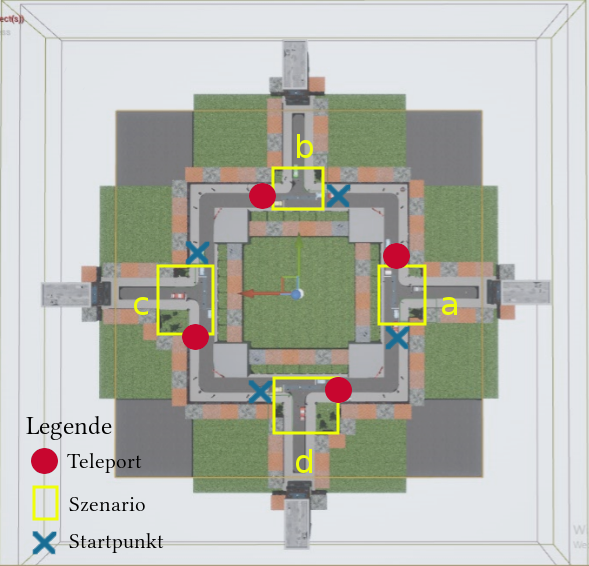
\includegraphics[scale=0.7]{../Bilder/mapLegende.png}
	\caption{Ansicht der Testumgebung von oben}
	\label{img:map}
\end{figure}


Abbildung \ref{img:map} zeigt die erstellte Karte von oben. 
Die Versuchsperson kann sich ausschließlich auf dem äußeren Fußgängerweg bewegen, sodass sie die vier Ampelkreuzungen überqueren muss. Die Laufrichtung ist gegen den Uhrzeigersinn vorgegeben.\\
Die gelben Kästen zeigen die Positionen der jeweiligen Szenarien an, die roten Punkte die Teleporter. Diese können untereinander beliebig verbunden werden, sodass verschiedene Szenarioreihenfolgen simpel und schnell umsetzbar sind.\\
Das blaue x zeigt die möglichen Einstiegspunkte, wobei es vom Startszenario abhängt, welcher tatsächlich aktiv ist. Die restlichen drei bleiben entsprechend passiv. Der zu erreichende Endpunkt liegt hinter dem letzten durchlaufenen Szenario. 

\begin{figure}[H]

	\subfigure[Ampelphase an einem LKW]{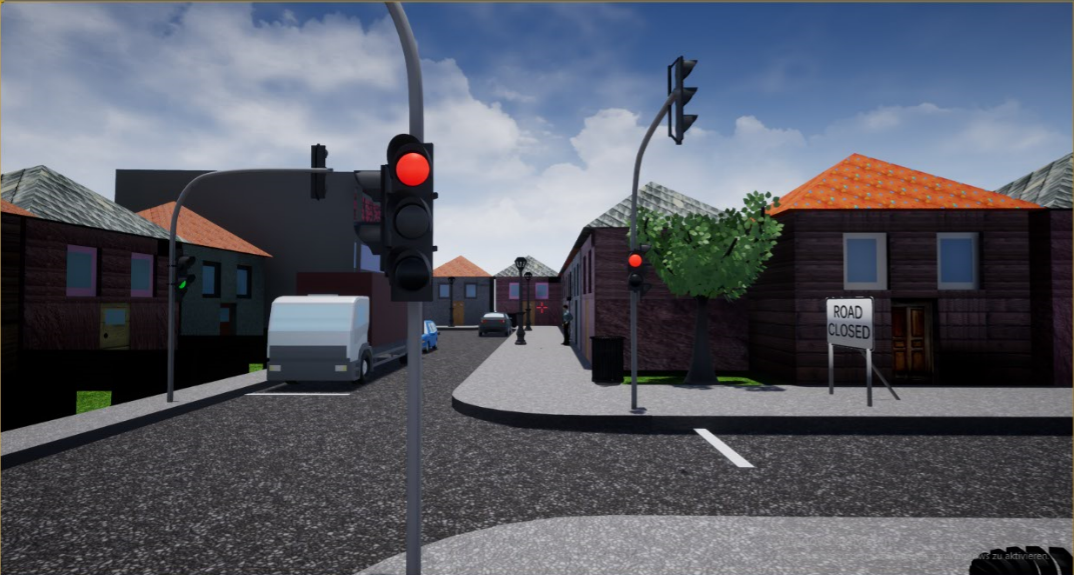
\includegraphics[width=0.5\textwidth]{../Bilder/a.png}}
	\subfigure[Ampelphase mit Vogel und Menschen]{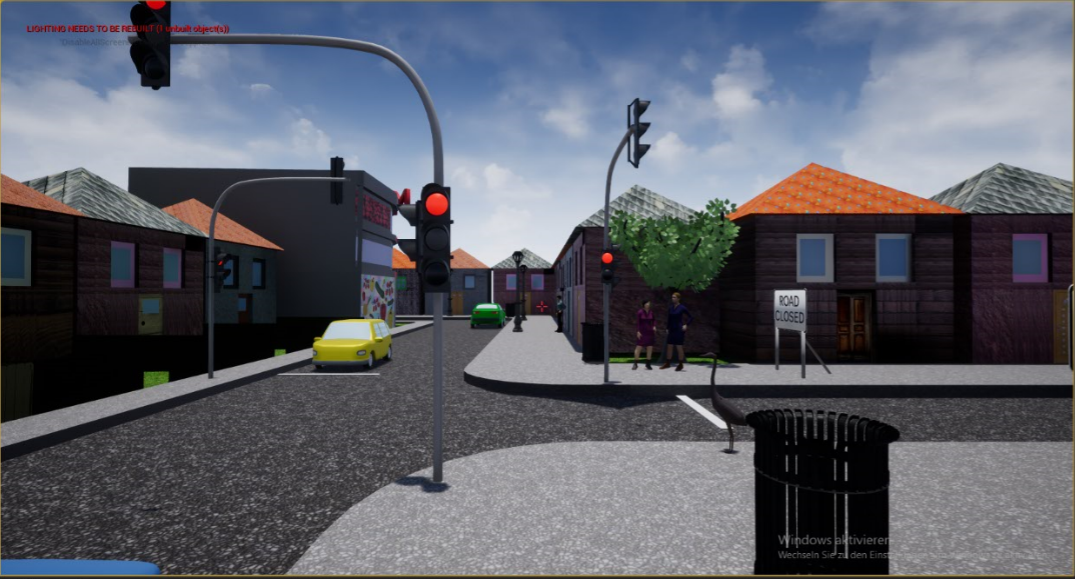
\includegraphics[width=0.5\textwidth]{../Bilder/b.png}}


	\subfigure[Ampel neben einem schaukelndem Kind mit rosa Shirt]{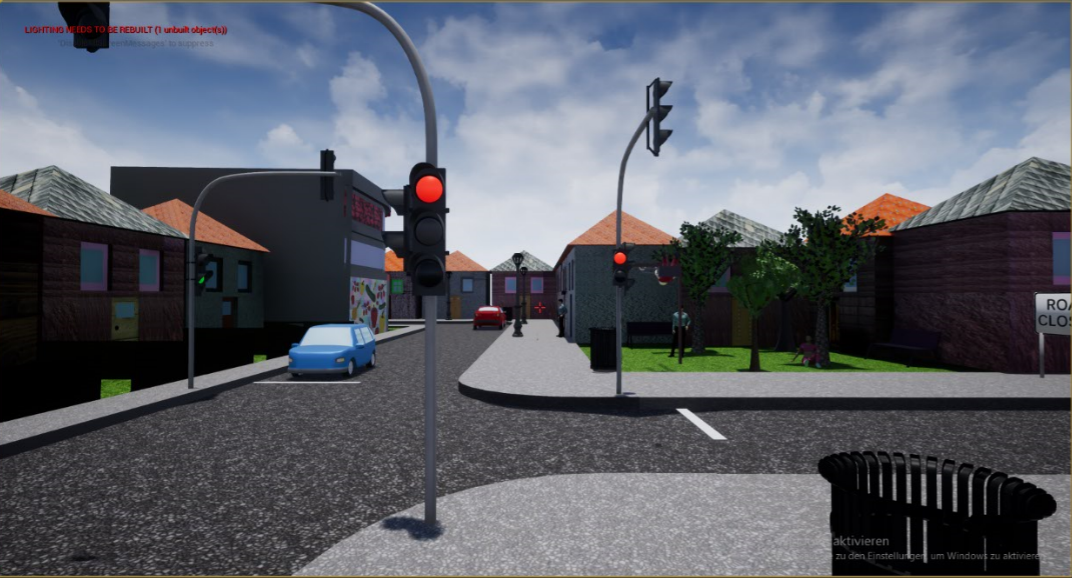
\includegraphics[width=0.5\textwidth]{../Bilder/c.png}}
	\subfigure[Ampel neben einem schaukelndem Kind mit grünem Shirt]{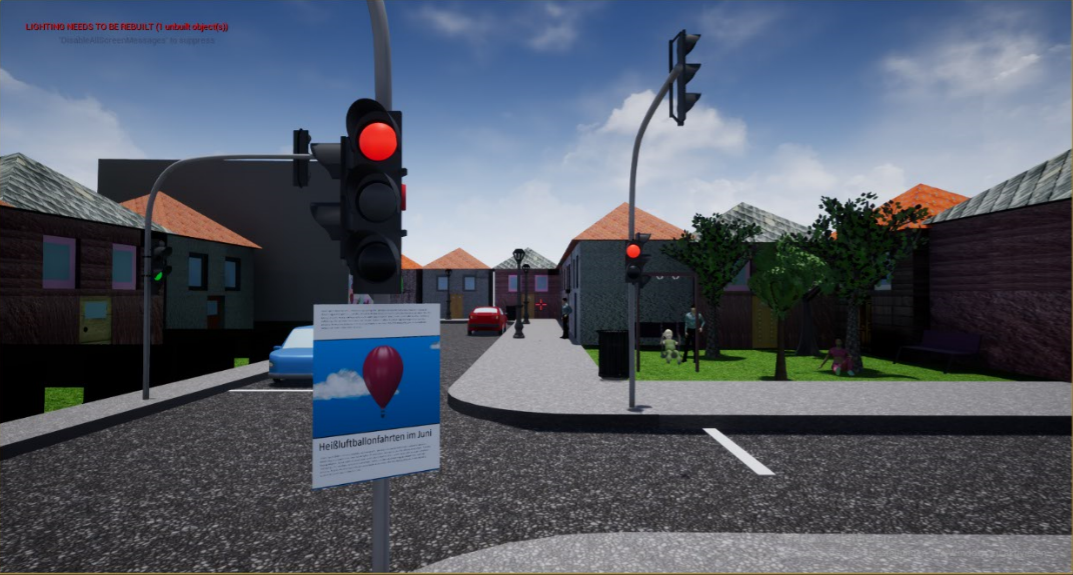
\includegraphics[width=0.5\textwidth]{../Bilder/d.png}}
	\caption{Benutzeransicht der Kreuzungen}
	
\end{figure}



Die auditive Manipulation wird durch ein gleichmäßig schnelles (Szenario \textbf{a}) oder langsames (Szenario \textbf{b}) Ticken der Fußgängerampel realisiert. Auffällige Objekte sollen der Versuchsperson helfen, sich an das jeweilige Szenario zu erinnern (ein LKW in Szenario \textbf{a} und ein Fischreiher auf dem Gehweg in Szenario \textbf{b}).\\
Ein schaukelndes Kind stellt die visuelle Manipulation dar, da es durch seine Animation den Eindruck macht schneller (Szenario \textbf{c}) oder langsamer (Szenario \textbf{d}) zu schaukeln als es in der Realiät möglich ist. Die Versuchsperson ist durch die Weltlogik dazu gezwungen an der Ampel zu warten, sodass das jeweilige Szenario auf sie wirken kann.
\label{subsec:aufbau}

\subsection{Software}
\subsubsection{Blender}
Blender wurde für das Erstellen der benötigten 3D-Objekte und zum Animieren der visuellen Zeitgeber verwendet.\\

% 3d objekte
\textbf{3D-Objekte}\\
Zu den verwendeten Objekten zählen die Ampeln, Autos, Bäume, Gärten, Gehsteige, Laternen, menschliche NPCs, Mülleimer, die Parkbank, das Plakat an der Ampel, der Fischreiher, die Schaukel, Straßenschilder, der Supermarkt und Wohnhäuser.\\
 Erstellt, aber nicht in der Testumgebung verwendet wurden die Blumen, Büsche, der Heißluftballon, der Hund, der Kaktus, die Rasenfläche, die Sonne, Straßen und -schilder und Wolken.\\
		Blumen, Büsche und die Rasenfläche wurden nachträglich entfernt, da diese Details zu viel GPU-Leistung forderten. Der Heißluftballon wurde indirekt in Form eines Fotos auf dem Plakat verwendet und für den Kaktus kein geeigneter Platz gefunden. Ebenfalls wurde aufgrund von Importproblemen des Hundes in die Unreal Engine stattdessen der bereits vorliegende Fischreiher verwendet und keine Zeit in die Fehlersuche investiert.
 		Sonne und Wolken waren in der Unreal-Vorlage bereits enthalten und mussten nicht durch die eigenen ersetzt werden. 
		Die Straße wurde durch eine Platte mit Straßentextur dargestellt, da sich dies als einfacher erwies und von den Straßenschildern wurden nicht alle benutzt, daher sind sie in beiden Listen wiederzufinden.\\
		
		
	

		\begin{figure}[H] % here - top - bottom - page, das ! erzwingt die Position falls möglich
			\centering
			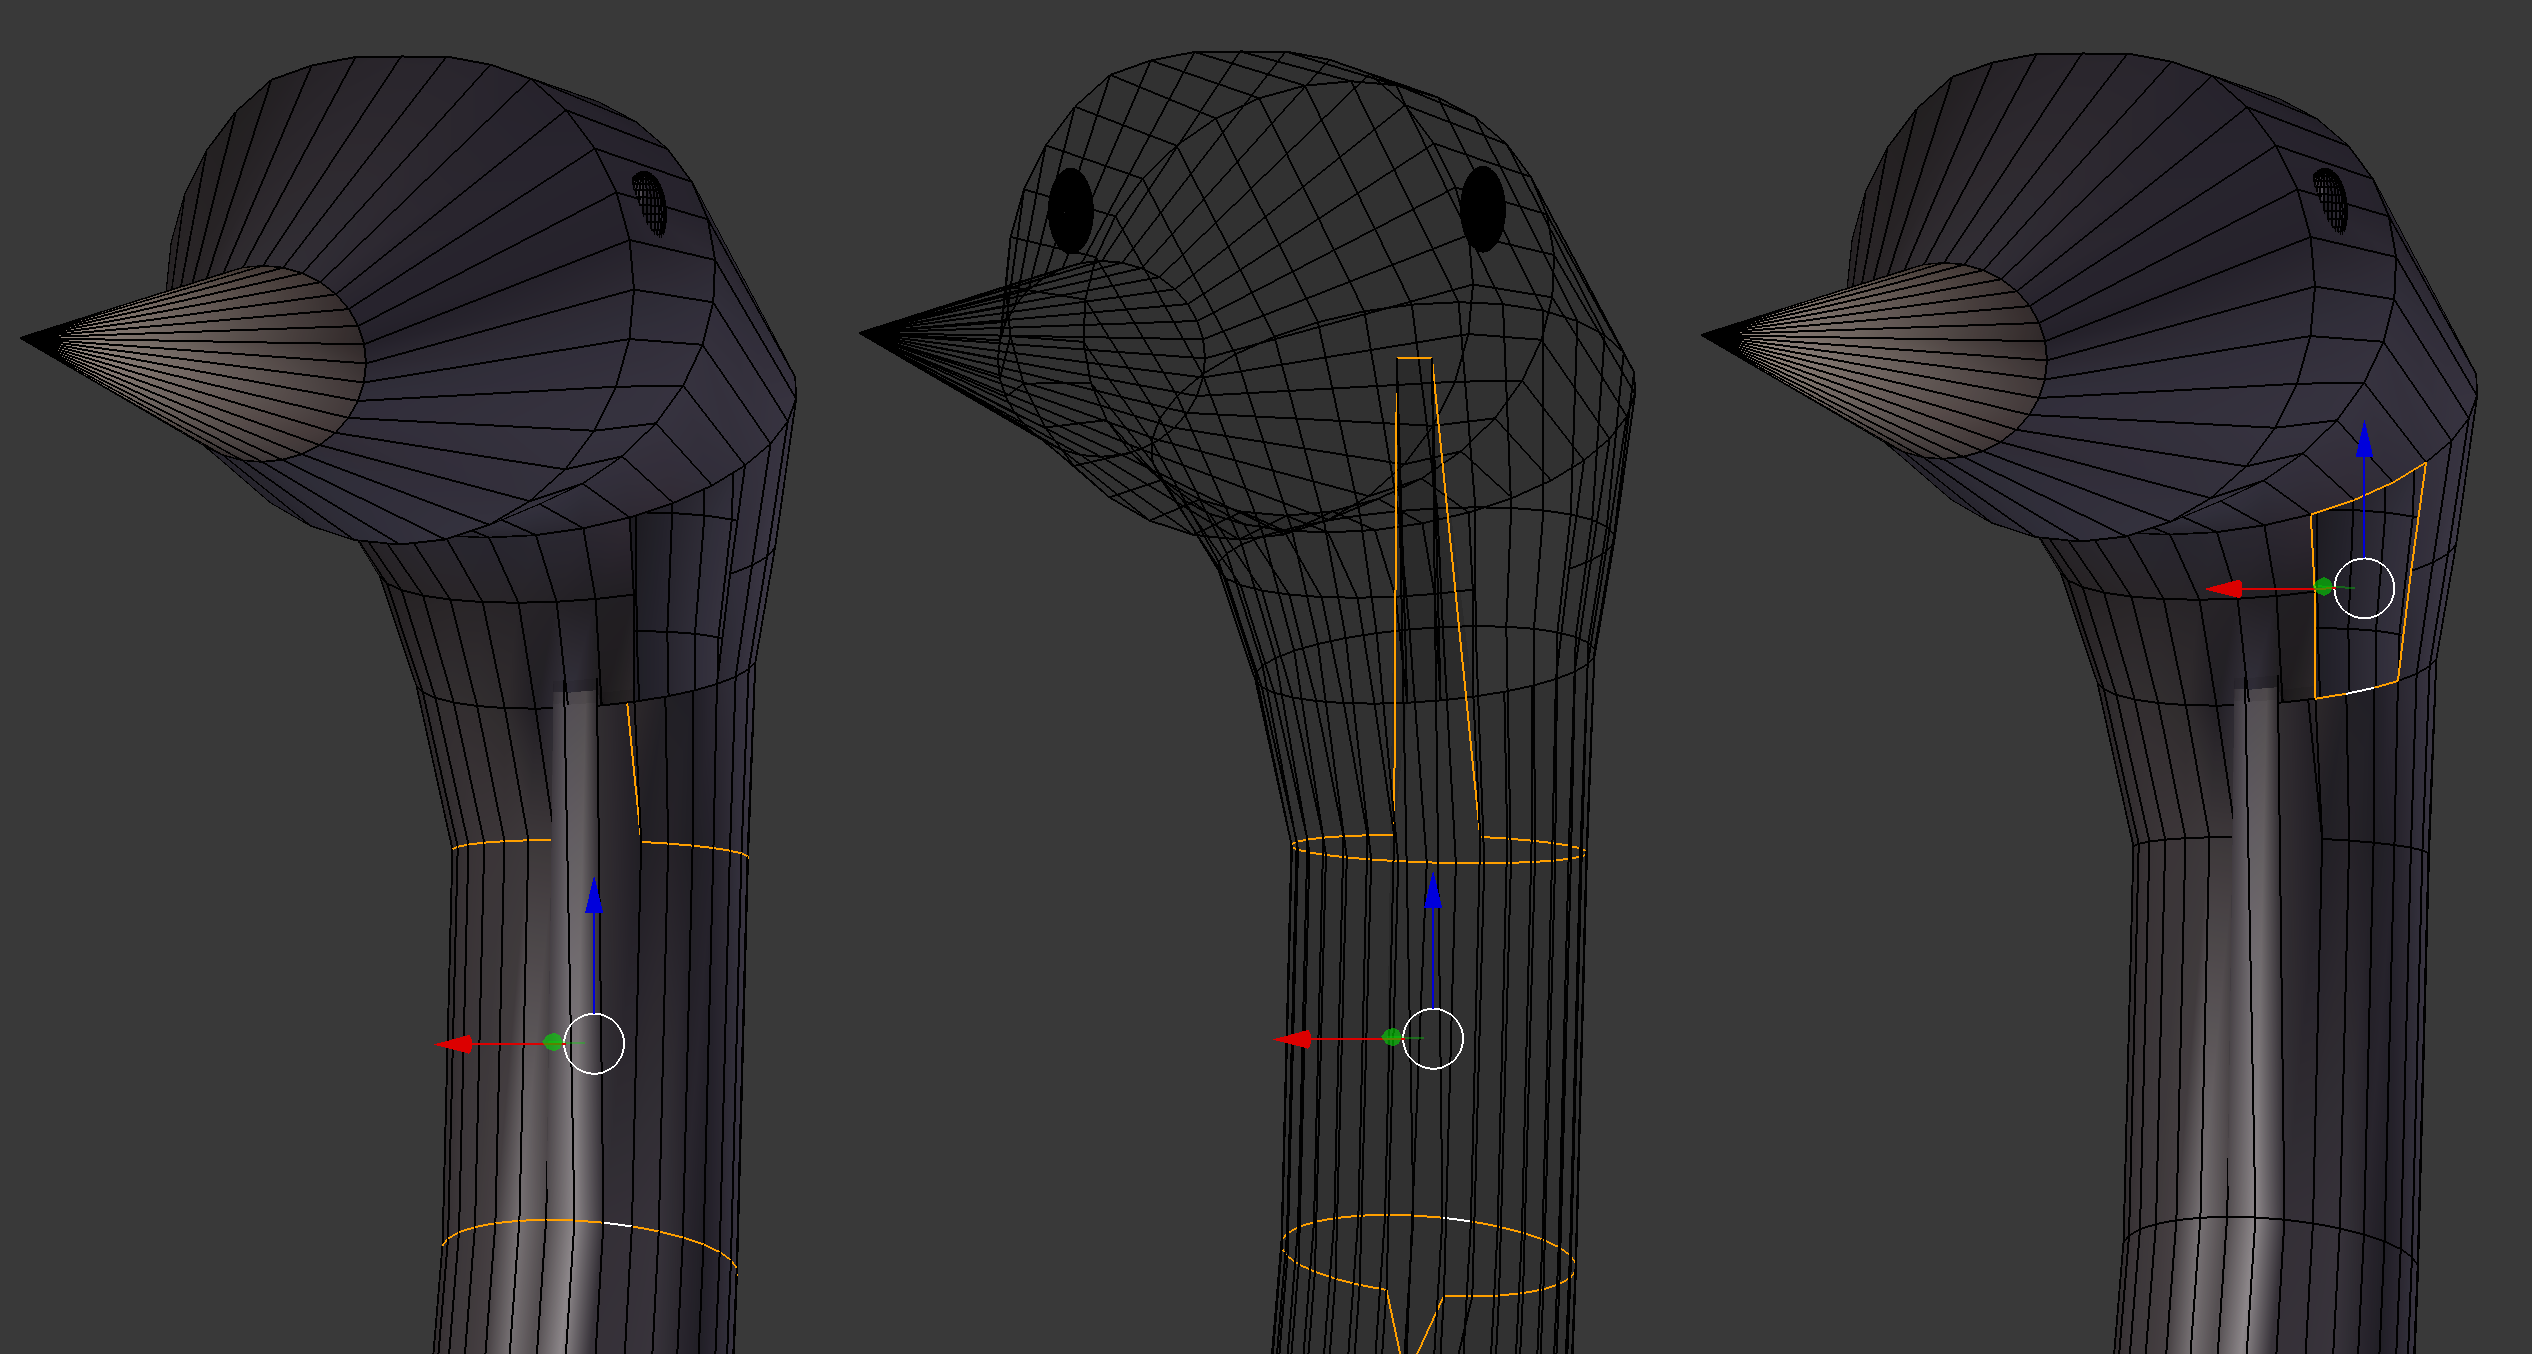
\includegraphics[height=\textheight, width=\linewidth, keepaspectratio, angle=0]{../Bilder/Heron_Problem.png} % trim - l u r o
			\caption{Nachträglich behobene Fehler in Blender}
			\label{img:heron-error}
		\end{figure}

An den erstellten Objekten traten gelegentlich kleinere Fehler auf, wie der in Abbildung \ref{img:heron-error} zu sehende Reiher, der nachgebessert werden musste. Zwei Punkte vom Hals waren fälschlicherweise bis in den Kopf verschoben, wodurch seitlich ein kleines Loch entstand. Diese Fehler konnten durch Verschiebungen der Punkte leicht behoben werden.\\
			 
\textbf{Keyframe-Animationen}\\
Die Animation der Schaukel als Zeitgeber wurde mit den in Blender integrierten Keyframes realisiert. Die Schaukelseile und der -sitz sind als ein Objekt fest miteinander verbunden und wurden um das statische Gerüst bewegt. Ausgangspunkt ist der höchste Punkt des Sitzes hinter Schaukel, welcher entsprechend weiterbewegt und als Keyframe in der Zeitleiste gespeichert wird, bis eine vollständige Schaukelbewegung animiert ist. Die Bewegung wurde einmal in Keyframes gespeichert und konnte für die schnelle und langsame Animation entsprechend gedehnt oder gestaucht und seperat gespeichert werden.\\
Die zur Schaukelbewegung passenden Bewegungen des Kindes wurden an der Figur mithilfe von Skelettanimationen und Keyframes realisiert und in die Schaukel-Datei importiert. Das Kind wurde im 3D-Raum entsprechend positioniert und die Keyframe-Zeitleisten aufeinander abgestimmt. \\
Da beim Unreal-Import Fehler in der Animation des Kindes auftraten, die nicht zeitnah behoben werden konnten, wurde in der finalen Version allerdings ein statisch auf der Schaukel sitzendes Kind verwendet. 
		
\subsubsection{Unreal Engine}
Ausgangspunkt der virtuellen Testumgebung war zunächst die VR-Vorlage, in welche die fertigen 3D-Objekte eingefügt wurden. Die passende Skalierung zu finden stellte sich zu Beginn als Herausforderung dar, da es in einer nahezu leeren Welt keine Orientierungspunkte gab. Nach einiger Recherche wurde ein Schachbrett mit je $1m^{2}$-großen Feldern unter die Map gelegt, an welcher sich die Platzierung der Straßen und Gehwege orientierte. Danach wurden Häuser, Gärten und die kleineren Objekte in die Welt eingefügt.
Die Implementierung der Ampelschaltung, der fahrenden Autos und der Teleporter waren die aufwendigsten Komponenten der Weltlogik, sodass auch viel Zeit in Fehlersuche und -behebung investiert werden musste. Sie wurden duch Blueprints implementiert.\\
		Durch die Umstellung der Steuerung auf herkömmliche Controller wurde etwa mittig im Designprozesses die anfänglich gewählte VR-Vorlage durch eine 3rd-Person-Vorlage ersetzt, da dies das Anschließen eines Controllers enorm vereinfachte.
				Im Laufe der Arbeit mit der Unreal Engine traten einige Fehler auf, deren Suche und Behebung teilweise sehr viel Zeit in Anspruch nahm.\\
Die Bearbeitungs-Ansicht (Texture) in Blender entsprach teils weder der in Blender gerenderten Ansicht (Rendered) noch der in der Unreal Engine angezeigten Ansicht, sodass teilweise drei verschiedene Texturansichten existierten und die Materials dieser Objekte nach dem Import in der Unreal Engine nachträglich bearbeitet werden mussten. Nahezu alle Materials wurden in der Unreal Engine editiert, da einige der in Blender definierten  Materialeigenschaften wie Specular Lightning oder Spiegelungen nicht von übernommen wurden.\\
Ebenfalls wurde bei einigen Objekten die Textur nicht korrekt dargestellt oder Objekte als teilweise durchsichtig. 
Die Textur einiger Objekte wurde nur angezeigt, wenn sich der viewpoint innerhalb des Objekts befand. Dies stellte sich bei näherer Betrachtung als ein Fehler an der Objektoberfläche heraus, der durch Inventierung der Normalen behoben werden konnte.		
Ein zentrales Problem war, dass jegliche von uns erstellten Objekte nach einem Build des Lightnings komplett schwarz waren. Nach einiger Recherche stellte sich heraus, dass alle in der Unreal Engine verwendeten Objekte zwei UV-Maps benötigen. Die zweite ist notwendig für das korrekte Darstellen des Lightning und ist, zumindest bei statischen Objekten, zwingend notwendig. Sich bewegende Objekte wie beispielsweise die Autos werden anders gerendert und benötigen diese zweite UV-Map nicht. 
		
		
				%Nach einiger Zeit stellte sich ebenfalls heraus, dass es für die Spiellogik einen erheblichen Unterschied macht, ob man die Welt mit der Oculus Rift durchläuft, oder "`auf dem Bildschirm''. Beispielsweise wird eine Triggerbox, die man betritt oder verlässt, normalerweise nur einmal getriggert. Beim Betreten/Verlassen mit VR-Ansicht hingegen um die zwanzig mal.
	%%%%%%%%%%%%%%% achtung relevant ?
	%_________________________________________________________________-				
				
				
				
				
				
	

			

			
		\begin{figure}[!htbp] % here - top - bottom - page, das ! erzwingt die Position falls möglich
			\centering
			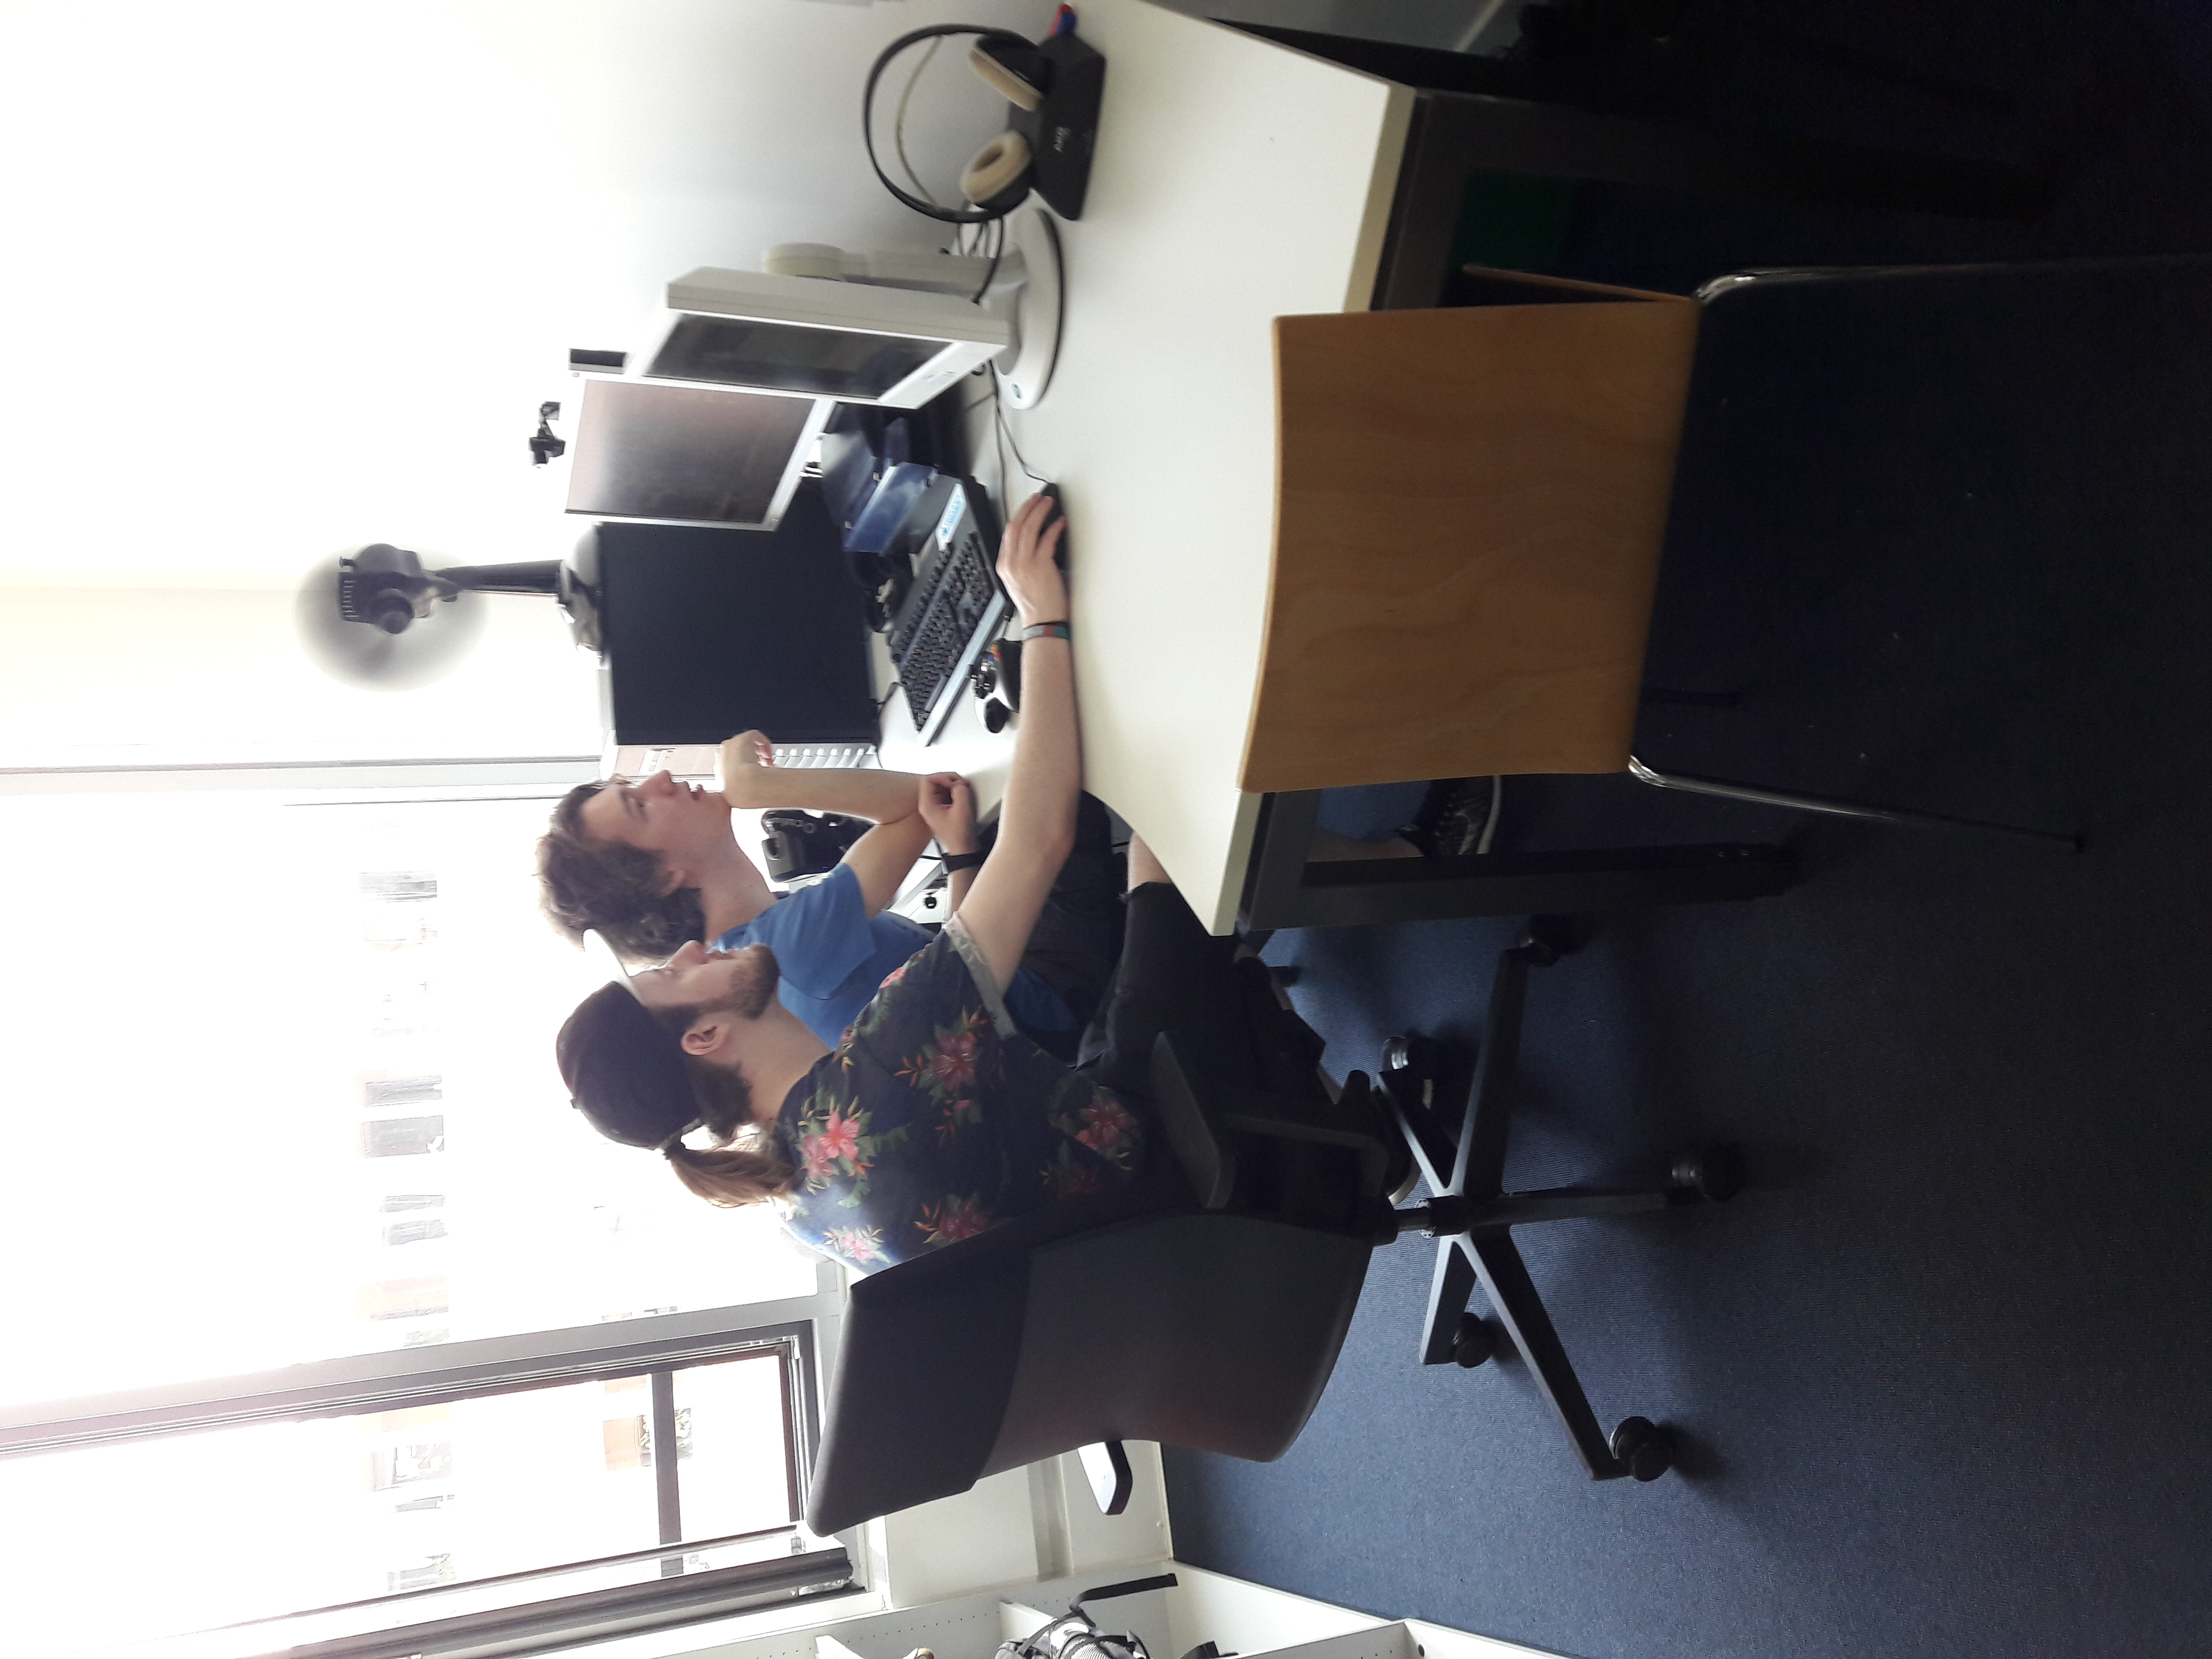
\includegraphics[trim = 200mm 0mm 600mm 0mm, clip, height=\linewidth, width=\textheight, keepaspectratio, angle=270]{../Bilder/20170619_102101.jpg} % trim - l u r o
			\caption{Problemlösung in Unreal}
			\label{img:porblemloesung}
		\end{figure}
		
		

\subsection{Hardware}
\label{subsec:hardware}
Folgende Hardware wurde für das den Versuchsdurchlauf verwendet: Ein LG Computer unter Windows 10, zwei Monitore (Fujitsu Siemens P19-1A \& 2. Benq FP222WH) auf denen die Versuchsleiter die Testumgebung beobachten konnten. Außerdem war der Raum mit Kopfhörern ausgestattet, um äußere Geräusche zu minimieren, sowie die Audio und Hintergrundgeräusche in der VR zu demonstrieren, die Oculus DK2 VR-Brille zur Orientierung in der VR und ein XBox-Controller für die Steuerung in der Welt.

\subsection{Probleme und Hindernisse}
Die Probleme, die das Projekt behinderten sind primär entweder organisatorischer oder technischer Natur.\\
Zeitliche Fehleinschätzungen zu Beginn des Experiments erwiesen sich als fatal, da die Termine zur Fertigstellung der einzelnen Arbeitsschritte im Verlauf des Projekts nicht mehr eingehalten werden konnten.
Erschwerend hinzu kamen die Inkompabilitätsprobleme der Oculus Rift und dem Computer der Virtusphere, welche den Projektfortschritt lahm legten und darin resultierte, dass bereits vereinbarte Termine mit Versuchspersonen verlegt werden musste. Weiterhin wurde die Virtusphere durch einen gewöhnlichen Controller ersetzt, da in der gegebene Zeit keine Lösung gefunden werden konnte.\\
	Während der Versuchsdurchführung schaltete sich teilweise die VR-Brille nach einer Weile ab. Dieses Problem trat allerdings nur sehr selten auf und konnte innerhalb von Sekunden behoben werden. Weiterhin war immer mindestens ein Mitglied des Technikteams während der VR-Phase anwesend und konnte bei Unstimmigkeiten eintreten, obwohl auch das Organisationsteam in die technische Bedienung eingewiesen wurde.\\
	Alle im Verlaufe des Projekts aufgetretenen Probleme konnte schlussendlich gelöst werden.
				

\section{Durchführung}
\subsection{Apparaturen}



Zwei Räume wurden für die Durchführung des Experiments genutzt. In  \textit{Raum 1} fanden alle Formalitäten, Fragebögen und Zeiteinschätzungstest sowohl vor als auch nach der VR statt. Zu den Materialen dieses Raumes gehören die Dokumente (siehe Kapitel \ref{subsec:dokumente}), ein Gerät zum Stoppen der Zeit, das Infrarot-Thermometer (Braun ThermoScan 7 Infrarot Ohrthermometer IRT6520) und die dazugehörigen Schutzkappen. Neben den in Kapitel \ref{subsec:hardware} genannten Apparaturen, wurde zusätzlich eine Stoppuhr genutzt. 


\label{subsec:dokumente}
\subsection{Dokumente}
Alle Ergebnisse einer Versuchsperson wurden auf Papier festgehalten, zusammengefasst gelagert und nach der des Projekts digitalisiert. Diese analoge Arbeitsweise wurde gewählt, um technische Probleme und Datenverlust zu vermeiden und da es für Versuchsleiter bei der hohen Anzahl an Versuchspersonen übersichtlicher und praktischer ist, alle zu einer Versuchsperson benötigten Dokumente physisch beieinander aufzubewahren.

\subsubsection{Einverständniserklärung}

Die Einverständniserklärung weist die Versuchsperson auf die allgemeinen Informationen, den Ablauf des Experiments und die Vertraulichkeit der Daten hin, nennt mögliche Risiken und Reaktionen des Körpers auf die VR und erinnert, dass das Experiment jederzeit abgebrochen werden kann. Jede Person, die am Experiment teilnehmen will, muss diese Einverständniserklärung unterzeichnen.

\subsubsection{Intelligenztest}
	
Um Intelligenz als Einflussfaktor auf Zeitwahrnehmung (vgl. Kapitel 1.3 im Paper) in den Ergebnissen berücksichtigen zu können, wurde ein Intelligenztest in den Experimentablauf integriert.
Mithilfe von Till Rackwitz, Masterstudent der Psychologie aus Hamburg und spezialisiert auf Intelligenztests, wurde der psychologisch anerkannte "`Mehrfach-Wortschatz-Intelligenztest (MWT-B)'', von Siegfried Lehre entwickelt und 1977 erstmals angewandt, in der fünften unveränderten Auflage für dieses Experiment ausgewählt. Er wurde aus der Testothek der psychologischen Abteilung der Universität Bremen ausgeliehen.\\
Aus 37 Wortreihen, welche jeweils aus vier erfundenen und einem deutschen Wort bestehen, gilt es das existierende Wort durchzustreichen, wobei der Schwierigkeitsgrad mit jeder Wortreihe steigt.\\
Der Test ist geeignet, da er das allgemeine Intelligenzniveau nach einem einfachen und zuverlässigen Schema misst, beliebig oft wiederholbar und für alle Versuchspersonen gleicht und ebenfalls kurz und simpel genug ist, um in den Experimentablauf integriert werden zu können. Ebenfalls benötigt dieser Test keine Versuchsleiter mit spezieller Ausbildung zur Abnahme von Intelligenztests. 
Da die Intelligenz im Zusammenhang mit Zeitwahrnehmung nur eine kleine Rolle spielt, reicht ein kurzer Test für dieses Experiment aus. 
\subsubsection{Fragebögen}
Durch das Verfahren des Fragebogens können Daten schnell und umfangreich erfasst und auf diese zu späteren Zeitpunkten zurückgegriffen werden. Jede Versuchsperson beantwortet unabhängig vom anwesenden Versuchsleiter die gleichen Fragen unter denselben Konditionen. Weiterhin werden Antworten sorgfältiger und ohne Zeitdruck beantwortet.\\

\label{subsec:fragebogen}
\textbf{Fragebogen A}

Die Versuchsperson wird auf mögliche Einflussfaktoren (vgl. Kapitel 1.3 im Paper) abgefragt, welche die Ergebnisse potenziell verfälschen könnten und berücksichtigt werden müssen.
\begin{itemize}
	\setlength{\itemsep}{0em}
	\item Stehen Sie unter irgendwelchen Drogeneinflüssen oder Medikamenten?
	\item Auf einer Skala von 1 bis 10, wie müde sind Sie? (1=nicht müde, 10=sehr müde)
	\item Haben Sie Ihnen bekannte Gehirnschäden oder psychische Erkrankungen?
	\item Ist Deutsch Ihre Muttersprache? Falls nein, welche Sprache ist Ihre Muttersprache?
	\item Möchten Sie das Experiment weiterhin durchführen?
\end{itemize}

\textbf{Fragebogen B}

Dieser Fragebogen wurde vom Versuchsleiter verwendet, um Ergebnisse der Zeiteinschätzungen und die Körpertemperatur zu notieren.\\


\textbf{Fragebogen C}

Hier werden Einschätzungen der Versuchsperson nach dem VR-Aufenthalt festgehalten.

\begin{itemize}
	\setlength{\itemsep}{0em}
	\item Sortieren der Szenarien/Ampelphasen vom kürzesten zum längsten mit Sekundenangabe. 
	\item Sortieren der Szenarien vom besten zum schlechtesten
	\item Wie lange hat der VR-Teil Ihrer Meinung nach gedauert?
	\item Hatten Sie Spaß?
	\item Ist Ihnen irgendetwas aufgefallen? Wenn ja, was?
	\item Haben Sie bemerkt, um was es sich in dem Experiment handelt? Wenn ja, worum handelt es sich und wann haben Sie es bemerkt?
\end{itemize}

\subsection{Ablauf}

%Bei der Experimentdurchführung nahmen jeweils im Durchschnitt 8.3 Versuchspersonen pro Tag an der Untersuchung teil. Jeder Durchlauf dauerte je nach Versuchsperson zwischen 35 Minuten bis 50 Minuten.
Der Ablauf des Experiments besteht aus drei Phasen: erste Zeiteinschätzungen und Intelligenztest (ca. 10 Minuten), die Navigation durch die virtuelle Testumgebung (ebenfalls ca. 10 Minuten) und die zweite Einschätzung (je nach Versuchsperson ca. 15-30 Minuten).\\
Das Technik- und Organisationsteam sind in diesem Abschnitt des Projekts anwesend. Jedes Teammitglied wurde im Vorfeld in den internen Ablauf eingewiesen und kann jeden Abschnitt des Experiments betreuen, wodurch der gesamte Ablauf flexibler gestaltet werden konnte.\\ 

\textbf{Phase 1}\\
Das Experiment beginnt mit der Versuchsperson und zwei Versuchsleitern in Raum 1. Einer der Versuchsleiter ist für den Durchlauf des Experiments verantwortlich, stellt der Versuchsperson die geforderten Aufgaben und unterhält sich ggf. mit ihr während des Zeiteinschätzungstests. Der zweite Versuchsleiter notiert die Ergebnisse und achtet auf einen fehlerfreien Ablauf. Die Versuchsperson erhält zunächst keine Einsicht in ihre Ergebnisse.\\
Der Versuchsperson wird die Einverständniserklärung ausgehändigt und darum gebeten, diese sorgfältig zu lesen und mit Namen und Datum zu unterschreiben, sollte sie weiterhin am Experiment teilnehmen wollen.
Der erste von insgesamt sechs Zeiteinschätzungstests wird durchgeführt (40 Sekunden ohne Gespräch), wobei keine Uhr als Hilfmittel benutzt werden darf.
Der Startpunkt wird vom Versuchsleiter vorgegeben sobald die Versuchsperson sich bereit fühlt und beendet sobald die Versuchsperson der Meinung ist, die gefragte Zeitspanne sei um.
Daraufhin wird ihr Fragebogen A ausgehändigt und darum gebeten, diesen sorgfältig auszufüllen.\\
Anschließend wird der Intelligenztest durchgeführt, wobei der Versuchspersonen die auf dem Papier vorgedruckten Instruktionen vorgelesen werden: 
,,hier instuktionen einfügen, keine zeitliche begrenung und keine hilfestellung''.\\
Im Anschluss wird ein weiterer Zeiteinschätzungstest  (40 Sekunden mit Gespräch) durchgeführt. Die Versuchsperson wird darauf hingewiesen, dass die gleichen Bedingungen wie beim zuvorigen Test gelten, sich einer der Versuchsleiter aber mit ihr unterhalten wird. Ist die Versuchsperson der Meinung, dass die zu schätzende Zeit vorüber ist, soll sie das Gespräch unterbrechen. Die Körpertemperatur der Versuchsperson wird mithilfe des Infrarot-Thermometers am Ohr gemessen und notiert.\\
Der letzte Zeiteinschätzungstest vor der VR wird durchgeführt (30 Sekunden ohne Gespräch). Die Bedingungen gleichen dem ersten Test.

\begin{figure}[H]
	\centering    
	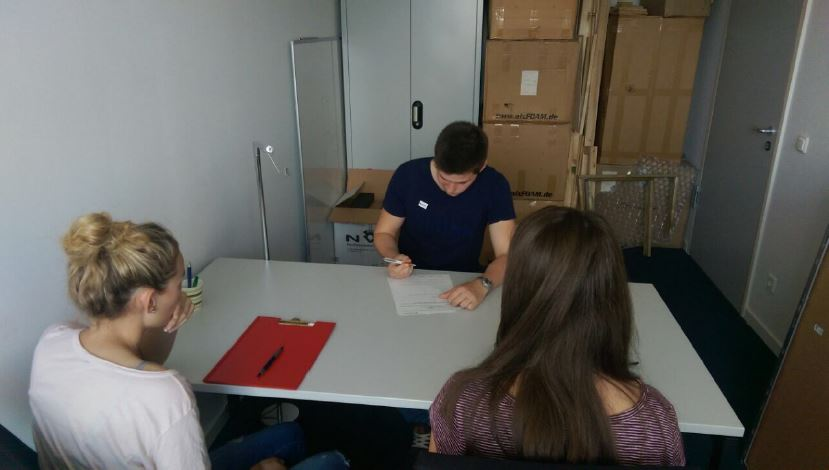
\includegraphics[height=\textheight, width=\linewidth, keepaspectratio]{../Bilder/t.jpg}
	\caption{Versuchsperson während der Befragung}
	\label{img:befragung}
\end{figure}

\textbf{Phase 2}\\ 
In Raum 2 befinden sich zwei weitere Versuchsleiter, wovon einer der Versuchsperson den weiteren Experimentverlauf in der VR erklärt und der zweite auf einen fehlerfreien Ablauf achtet.\\
Der Versuchsperson wird, nachdem sie auf dem Drehstuhl vor dem Computer platzgenommen hat, die Oculus Rift aufgesetzt, auf welcher die virtuelle Testumgebung bereits läuft. Sobald die Brille angenehm sitzt und die Versuchsperson ihre VR-Umwelt gut erkennen kann, bekommt sie die Anweisungen durch den Versuchsleiter. 
Die Handhabung des Controllers (mit welchem Knopf man sich fortbewegt und umschaut) und der Brille (man kann sich auch durch Kopfbewegungen umschauen) wird erklärt und die Versuchsperson auf die Regeln innerhalb der Testumgebung aufmerksam gemacht (es gibt einen zu erreichenden Endpunkt, Gehwege dürfen nicht verlassen werden, es gibt eine vorgesehene Laufrichtung, allgemeine Verkehrsregeln wie das Warten an einer roten Ampel müssen beachtet werden).  

Die Versuchsperson darf die Steuerung vor Beginn kurz testen. Ihr werden die Kopfhörer aufgesetzt und die Zeit bis zum Erreichen des vorgesehenen Endpunkts durch einen der Versuchsleiter gestoppt.
Sollte etwas nicht korrekt ablaufen, können die Versuchsleiter dies über den Monitor des Computers erkennen und in das Geschehen eingreifen.

\begin{figure}[H]
	\centering    
	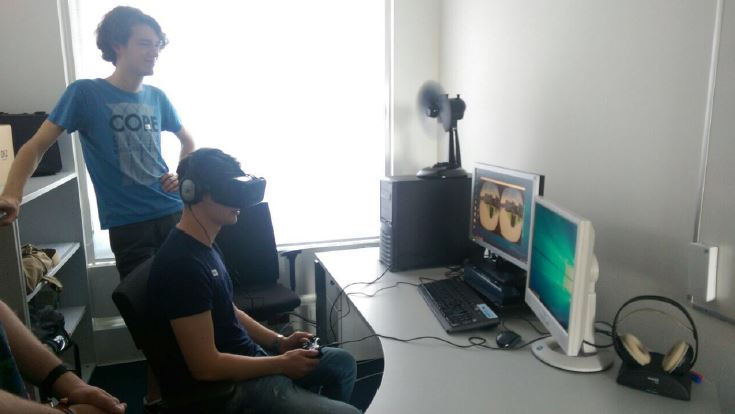
\includegraphics[height=\textheight, width=\linewidth, keepaspectratio]{../Bilder/v.jpg}
	\caption{Versuchsperson während der VR-Phase}
	\label{img:versuchsperson-in-vr}
\end{figure}

\textbf{Phase 3}

Zurück in Raum 1 schätzt die Versuchsperson ein weiteres Mal die Zeit ab (40 Sekunden ohne Unterhaltung), wobei die Anweisungen diesbezüglich aus Phase 1 erhalten bleiben. Die Versuchsperson füllt Fragebogen C aus (genaueres im Kapitel \ref{subsec:fragebogen}) und schätzt noch zweimal unter gleichbleibenden Bedingungen aus Phase 1 die Zeit ab (40 Sekunden mit Gespräch und 30 Sekunden ohne Gespräch) bevor das Experiment beendet ist. Die Versuchsperson hat die Möglichkeit ihre Testergebnisse, sowie die Punktzahl des Intelligenztests zu erfahren.


	\section{Versuchspersonen}
Für die Durchführung des Experiments warben wir Versuchspersonen an, um die Hypothesen empirisch zu überprüfen.
\todo{versuchsdesing, empirik etc} 
Diese waren bezüglich der Forschungsfrage unwissend und unterschrieben vor der Teilnahme eine Einverständniserklärung, die sie auf mögliche Risiken und datenschutzrechtliche Informationen (welche) aufmerksam machte. Alle Versuchspersonen nahmen freiwillig am Experiment teil und wurden nicht entschädigt. 

\subsection{Demografische Angaben}
Es wurden Versuchspersonen zwischen 18 und 80 Jahren gesucht, wobei eine 17-jährige Person mit der Einverständnis eines \textbf{erwachsenen?} ebenfalls am Experiment teilnahm. Das Durchschnittsalter aller Versuchspersonen liegt bei 31 Jahren. Vorerfahrungen im Bezug auf VR wurden bei der Suche nicht berücksichtigt.
%da die Zeitwahrnehmung von Jugendlichen langsamer ist als die von Erwachsenen. Der Grund: Je mehr Neues und Emotionales man erlebt, desto mehr prägt es sich im Gedächtnis ein; und desto länger wirkt ein Zeitraum im Nachhinein. Das ergab die Studie "`Age effects in perception of time'' von Marc Wittmann und Sandra Lehnhoff aus dem Jahr 2005 \cite{AgeEffects}. Aufgrund dessen wurden ausschließlich erwachsene Versuchspersonen gesucht, die über dem Zeitraum der "`erste Male erleben'' hinaus sind. 

Insgesamt wurden 48 gültige Ergebnisse für die Auswertung benötigt, 

%da die vier Szenarien in vierundzwanzig verschiedenen Reihenfolgen dargestellt werden konnten. Diese sollten jeweils von zwei Personen durchgeführt werden. Deshalb haben wir 50 Versuchspersonen eingeladen, um am Experiment teilzunehmen. Falls es während des Expriments zu Ausfällen kommen sollte oder Ergebnisse unbrauchbar wären, hatten wir zwei Versuchspersonen zusätzlich. \\

Die Verteilung der Geschlechter war nicht ausgeglichen, da sich überwiegend männliche Versuchspersonen bewarben. Ebenfalls lagen \textbf{xy} usw usf intelligenzverteilung \\


- beachte krankheiten + muttersprachler
- antal och uteslutna personer 
%Das gilt auch für den Bildungsstand der Versuchspersonen 

%Die Sprachkenntnisse waren uns dennoch wichtig, aufgrund des Mehrfach-Wortschatz Intelligenztests der auf guten Deutschkenntnissen basiert und wir die selben Voraussetzungen bei allen Versuchspersonen gewährleisten wollten. 

Weitere Voraussetzung, die nach Eingang der Bewerbung erfragt wurde, waren eine normale bzw. durch eine Brille oder Kontaktlinsen korrigierte Sehkraft und Farbsehen. 

\subsection{Suche}
\todo{überhaupt mal orga und technik definieren}
Das Organisationsteam war für die Suche der Versuchspersonen verantwortlich. Die Kommunikation zwischen Versuchspersonen und Team verlief über eine speziell erstellte E-Mail-Adresse. Meldeten Personen Interesse am Projekt an, wurde für sie in vorher eingeteilten Terminslots, welche sich über einen Zeitraum von sechs Tagen erstreckten, ein passender Termin gefunden.
\todo{und wieder umgetragen}
Die meisten Versuchspersonen wurden über eine Anzeige auf der Website \textit{ebay-kleinanzeigen.de} auf dieses Projekt aufmerksam. Die Annonce wurden mehrmals in der Woche aktualisiert, sodass sie eine Großzahl von Menschen sehen konnte.\\
Versuchspersonen im Bekanntenkreis anzuwerben war die zweiterfolgreichste Methode. Es wurde sich darauf geeinigt, keine Personen des engeren Familien- oder Freudeskreises teilnehmen zu lassen, da diese über Vorwissen der Forschungshypothese verfügen könnten oder sich aufgrund der emotionalen Bindung zu einem der Versuchsleiter ,,viel Mühe'' geben.\\
Auf die in der Universität Bremen verteilten Flyer kamen die wenigsten Rückmeldungen. Es wurde der gleiche Text wie in der Internetannonce verwendet:\\

\par
\begingroup
\leftskip4em
\textbf{Freiwillige Versuchspersonen für VR-Experiment gesucht}

Bist du im Alter zwischen 18 und 80, bist fit und hast Lust mal in eine virtuelle Welt einzutauchen? Dann bist du genau die richtige Person, um an unserem Experiment teilzunehmen!

Wir sind eine Gruppe von Studierenden aus dem Bereich Digitale Medien an der Universität Bremen und führen im Rahmen unseres Bachelor-Projekts eine Untersuchung zur Wahrnehmung in der virtuellen Realität. Mit einer sogenannten Virtual Reality Brille schicken wir dich in eine andere Welt in der du verschiedene Szenarien auf dich einwirken lässt.

Wenn du Interesse hast uns bei unserem Experiment zu unterstützen, dann würden wir uns über eine E-mail von dir freuen. Nenne uns bitte in deiner Nachricht deinen Namen, Alter, Geschlecht sowie die Tage an denen du zur Verfügung stehst für das VR Experiment - an folgende Adresse: experiment.sose17@gmail.com \\

Unser Experiment werden wir an diesen 6 Terminen durchführen: \\

Mo 19., Mi 21., Do 22., Fr 23., Sa 24. und Mo 26. Juni 2017 immer jeweils zwischen 10 und 18 Uhr, im Cartesium an der Universität Bremen. Die Dauer wird 30 Minuten bis 45 Minuten betragen.

Wir freuen uns auf hoffentlich zahlreiche Nachrichten!

Das ¡Experiment! Projekt Team
\par 
\endgroup


\subsection{Ethik}
Die Untersuchung menschlichen Verhaltens mit dem Ziel an Forschungsergebnisse zu gelangen ist problematisch, wenn Gefahr besteht, dass die Manipulation die Persönlichkeit eines Menschen langfristig prägt oder beeinflusst.\\
 Bereits zu Beginn wurden Ideen verworfen, da sie aufgrund moralischer Bedenken für dieses Projekt ungeeignet schienen (vgl. Kapitel \ref{subsec:ideenfindung}). Obwohl ein Forschungsinteresse seitens des Teams bestand, überwiegte die Skepsis, ob den Versuchspersonen moralisch fragwürdige Szenarien zugetraut werden können. Auch wenn es anfänglich unbewusst geschah und sich erst zu nach der Versuchspersonenphase mit der Frage der ethischen Vertretbarkeit beschäftigt wurde, wurde sich während des ganzen Experiments an persönliche moralische Richtlinien gehalten. \\
Die Sicherheit der Versuchspersonen war zu jedem Zeitpunkt gewährleistet, da sie über den Ablauf des Verfahrens und die möglichen Unannehmlichkeiten und Risiken im Vorfeld informiert wurden. Durch die Einverständniserklärung, übernahmen die Versuchspersonen die persönliche Verantwortung und somit auch die Risiken in Kauf. Des Weiteren wurden sie zu Fragen ermutigt, um Zweifel oder Missverständnisse zu vermeiden. Alle Ergebnisse werden vertraulich und unter Ausschluss der Öffentlichkeit behandelt und pseudonymisiert.

\section{Ergebnisse}
Auf die Ergebnisauswertung des Experiments wird in der wissenschaftlichen Ausarbeitung eingegangen.
\section{Diskussion}
Die darauffolgende Diskussion wird ebenfalls nur in der wissenschaftlichen Ausarbeitung behandelt.


\section{Fazit} % Autor: Chovi
%\subsection{Zusammenfassung}
%Wie bereits vorgestellt, lautet unsere Forschungshypothese: "`Kann man das Zeitempfinden in der Virtuellen Welt durch bestimmte Zeitgeber manipulieren?''.
%Um dies zu beantworten haben wir unsere eigene Virtual Reality entwickelt und die von uns ausgewählten auditiven und visuellen Zeitgeber integriert. Von beiden Varianten gab es je zwei Ausführungen, eine langsame von der wir erwartet haben, dass sie zeitdehnend auf die Wahrnehmung der Versuchsperson wirkt und eine schnelle die zeitverkürzend wirken soll. Unsere VR-Welt bestand aus vier Kreuzungen und jeder von diesen wurde ein Zeitgeber zugeteilt. Während unsere Versuchspersonen an der Ampel der jeweiligen Kreuzung warteten, waren sie diesen Zeitgebern ausgesetzt. 

%Wie zuvor im Paper beschrieben, wurden vor der VR  die für uns relevanten Daten der Versuchsperson gemessen und aufgenommen, darunter Körpertemperatur, Intelligenz und Müdigkeit. Die Befragung nach der VR bezog sich dann überwiegend auf die Wahrnehmung der eben erwähnten vier Szenarien, mit dem Hauptaugenmerk auf die empfundene Dauer dieser. Mithilfe unserer Ergebnisse wollten wir herausfinden, ob unsere Hypothese, dass das Zeitempfinden in der VR durch gewisse Zeitgeber gezielt beeinflusst werden kann, belegbar ist.

\subsection{Schlüsselergebnisse}
	\begin{enumerate}
		\item Es lässt sich im Rahmen dieses Experiments nicht bestätigen, dass Faktoren wie Alter, Körpertemperatur, Intelligenz und Müdigkeit die Zeiteinschätzung beeinflussen
		\item Es fällt Versuchspersonen leichter, kurze Zeitspannen (30 Sekunden) zu schätzen als längere (40 Sekunden)
		\item Ablenkungen in Form eines Gespräches, verschlechtern das Ergebnis, da die Zeit als deutlich länger geschätzt wird 
		\item Zwischen auditiven und visuellen Zeitgebern ist kein deutlicher Unterschied bezüglich der Wirkung zu verzeichnen
		\item Laut den Ergebnisse dieses Projekts hat die VR keinen so starken Einfluss auf die Versuchspersonen, dass es bemerkenswerte Unterschiede zwischen den Zeitschätzungen vor und nach der VR gibt.
		\item Die Hypothese, dass durch schnelle Zeitgeber die subjektive Zeit der Versuchspersonen entsprechend zügiger vergeht, kann bestätigt werden. Der geschätzte Durchschnittswert liegt  deutlich unter der tatsächlichen Dauer des Szenarios.
		\item Die Hypothese, dass durch langsame Zeitgeber die subjektive Zeit der Versuchspersonen entsprechend langsamer vergeht, kann in dem Sinne bestätigt werden, dass die "`Langsamen'' als deutlich länger geschätzt werden, als jene Szenarien mit den schnellen Zeitgebern. Dennoch werden diese nicht länger geschätzt als sie tatsächlich gedauert haben.
	\end{enumerate}

\subsection{Nutzen der Arbeit}
Verständlicherweise nützt unsere Arbeit Forschenden, die sich mit der VR auseinandersetzen. Der Bekanntheitsgrad der VR steigt und diese wird stetig weiterentwickelt. Dementsprechend werden sich Menschen auch länger in der VR aufhalten. Alles wird realer wirken müssen und Gesetze oder Konzepte, die wir aus unserer Realität kennen, werden dort von Menschenhand kontrolliert werden können. Die Zeit wird dabei auch eine Rolle spielen und somit die Zeitgeber. Sinnvoll zu wissen ist es, was hier bei der Umsetzung beachtet werden muss, wie diese Umweltfaktoren auf die VR-Besuchenden wirken und ob oder welche Unterschiede es zur Wahrnehmung realer Zeitgeber gibt. Die Vorstellung, dass in Zukunft Zeitgeber in der VR derart manipuliert werden können, dass es dem VR-Besuchenden vorkommt er wäre, beispielsweise mehrere Stunden in der Welt gewesen, wobei es in Echtzeit 15 Minuten waren, ist doch sehr beeindruckend. Man könnte in einer menschgeschaffenen weiteren Dimension, in weniger Zeit mehr erleben.

Unabhängig von der Forschung der VR ist die menschliche Zeitwahrnehmung selbst noch sehr unerforscht. Diese in der VR zu testen kann neue Perspektiven öffnen und zu Erkenntnissgewinn beitragen. Ähnlich wie auch die Entwicklung kreativer Computersysteme dazu beiträgt,  das Konzept der menschlichen Kreativität besser verstehen zu können \cite{comp}.

%\subsection{Aufbauende Arbeiten}

\label{subsec:kritik}
\subsection{Methodenkritik}

Bei Auswertung des Experimenablaufs fallen verschiedene Dinge auf, die anders hätten behandelt werden können.\\
Die Versuchspersonen darum zu bitten, nach der VR die Szenarien zeitlich einzuschätzen ist problematisch, da sich die Versuchsperson an etwas erinnern sollte, dem sie während der VR möglicherweise keine Aufmerksamkeit geschenkt hat.
 Es ist entsprechend schwierig nach der VR die Länge der Szenarien einzuschätzen, selbst wenn die Szenarien in Fragebogen C beschrieben waren. Einige Versuchspersonen gaben zu, dass sie teilweise nicht mehr wussten, von welchem Szenario die Rede ist und eine Antwort geraten haben. Das wiederum führt zu Ungenauigkeiten im Datensatz. 
 Besser wäre es gewesen während des VR-Aufenthalts und direkt nach Erleben des Szenarios die Zeiteinschätzung zu erfragen. Hierbei könnten die Versuchspersonen allerdings verstehen, worum es geht und bei der nächsten Ampel die Sekunden zählen. Das wäre auch nicht optimal, aber eine bessere Option als die von uns gewählte.\\
Die Zeitgeber hätten auch durch eine minimalistischer gestaltete Testumgebung (sowohl im Bezug auf verwendete Objekte als auch auf Farbgebungen) mehr in den Fokus der Aufmerksamkeit gerückt werden können.\\
Ein weiteres Manko sind auf Fragebogen C ungünstig gewählte Intervalle (0-7, 7-15, 15-25, 25-35 und länger als 35 Minuten) zur Frage, wie lange die Versuchsperson glauben in der VR gewesen zu sein. Diese Zeiten beziehen sich noch auf den Experimentablauf in der Virtusphere und wurden nicht an die neuen Umstände angeglichen. 
Kürzere Zeitintervalle hätten unter den aktuellen Umständen präzisere Ergebnisse liefern können. 70\% haben angegeben, sich 0-7 Minuten in der VR aufgehalten zu haben, was bei der Größe der Welt und der Geschwindigkeit, mit der man sich mit einem Controller darin bewegen kann, recht vorhersehbar ist und kein Wert mit großer Aussagekraft ist.\\
%Weiterhin fällt auf, dass wenn der Spaßfaktor gemessen wird, etwas in die VR integriert sein sollte, das auch Spaß bringt. Beispielsweise ein kleines Spiel oder Ähnliches, denn lediglich an der Straße längs zu gehen ist in der Welt vielleicht interessant, bewirkt aber wahrscheinlich nicht so viel spielerisches Vergnügen, sodass der Einfluss auf unsere Ergebnisse groß  genug ist. \\
%Der Aufbau der Testumgebung mag durch die immer gleich aussehenden Ecken monoton gewirkt haben, allerdings war dies die einfachste und effektivste Möglichkeit die verschiedenen Szenarioreihenfolgen zu implementieren.\\
Weiterhin wäre eine höhere Anzahl von Versuchspersonen besser für die Aussagekraft der Ergebnisse gewesen, war allerdings aus zeitlichen Gründen nicht umsetzbar.

\subsection{Folgearbeiten}
Es gibt verschiedene Möglichkeiten, methodisch auf dieser Arbeit aufzubauen und sie weiterzuentwickeln.

Eine Möglichkeit ist es, den Zeitraum des Aufenthalts zu verlängern und mehr Zeitgeber zu integrieren. Die Konfrontation der Versuchspersonen mit diesen kann dann nicht nur in einer Situation, beziehungsweise einem Szenario erfolgen, sondern während des gesamten Aufenthalts in der VR. Die dargestellte Umwelt spiegelt die jeweilige Geschwindigkeit wieder. Bestenfalls sollte man die Testperson zur Interaktion auffordern, so wie wir es uns auch am Anfang der Ideenfindung vorgestellt haben, bevor wir es aus zeitlicher Begrenzung der Umsetzung vereinfachen mussten. Nach dem Aufenthalt könnte man prüfen, ob der Versuchsperson die Abläufe in der Realität langsamer erscheinen. Wenn dies der Fall ist, sollte man messen wie lange es dauert, bis die Wahrnehmung sich wieder normalisiert und wenn das Know-how besteht, Nachforschungen darüber anstellen, welche Strukturen sich im Gehirn verändert haben. Dies wäre auch ein weiterer Ansatz, menschliche Zeitwahrnehmung zu verstehen.

Außerdem könnte man versuchen, langsame und schnelle Zeitgeber zu  kombinieren, um zu schauen, ob die zur Reizüberflutung und Überforderung führt oder ob so etwas wie ein "`inneres'' natürliches Zeitgefühl durch nicht eindeutige Beeinflussung bestehen bleibt.

Das Gebiet im Gehirn, dass das Empfinden der Zeit reguliert, wurde von den Wissenschaftlern vom Medical College of Wisconsin in Milwaukee und des Veterans Affairs Medical Center in Albuquerque entdeckt. Es handelt sich um die Basalganglien, einer funktionellen Einheit von Kerngebieten im Gehirn, die der Bewegungskoordination dienlich sind. Ginge man davon aus, dass sich die Zeitwahrnehmung durch die VR signifikant verändern lassen könnte, dann wäre es vielleicht möglich krankhaft falsch funktionierende Zeitwahrnehmung, wie sie etwa bei den Aufmerksamkeitsdefizitsyndrom - Patienten gegeben ist, mit regelmäßigen VR-Besuchen zu behandeln. Unter der Voraussetzung, dass es  möglich ist, durch regelmäßigen Aufenthalt in der VR die Struktur der Basalganglien zu beeinflussen, könnten diese Störungen möglicherweise verbessert werden.

 
Weiterhin gibt es da noch das auf unserem aufbauende Projekt von Mert Özenen. Dieses wird einen ähnlichen Ablauf wie unseres haben, nur das zusätzlich Umweltfaktoren, wie z.B. Sonne und Wind, durch entsprechende Beleuchtung und einem Ventilator simuliert werden.


	


\section{Abschließende Gedanken} % Autor: Jana, überarbeitet: Jana
Autor: Jana, Überarbeitung: Jana
	Wir sind in den verschiedenen Phasen des Projekts auf unterschiedliche Probleme gestoßen, von denen wir viele zeitnah lösen konnten. Allerdings gab es auch schwerwiegendere, deren Lösung für uns nicht gleich oder gar nicht offensichtlich war und die unseren ursprünglichen Zeitplan infolgedessen ungewollt stark beeinflusst haben.
	Durch die Inkompatibilität der Oculus Rift und dem Computer der Virtusphere konnten wir unser Projekt nicht wie ursprünglich geplant in der Virtusphere stattfinden lassen und mussten auf herkömmliche Controller ausweichen. Diese Umstellung ist sehr ärgerlich, da viel Zeit in die Problemlösung investiert wurde und wir den Versuchspersonen letztendlich doch nicht das bieten konnten, mit dem wir sie ursprünglich geworben hatten. 
Weiterhin zu kritisieren wäre eine nicht ganz ideale Arbeitsteilung, wodurch es gerade am Ende zu erheblichem Zeitverzug kam. Insbesondere das sog. \textit{Technikteam}, welches primär für die Erstellung der Blenderobjekte, das Einsetzen und das Animieren der Welt verantwortlich war, hat gleich zu Beginn des Projekts anstehende Aufgaben nicht sinnvoll verteilt. Alle Mitglieder waren gleichermaßen nur mit aktuellen Aufgaben beschäftigt, d.h., dass zunächst jeder für die Erstellung von Blenderobjekten verantwortlich war und so Kapazitäten und Zeit verschwendet wurde, da sich bisher noch keiner besonders gut mit der Software auskannte und sich alle gleichermaßen neu einarbeiten mussten. \\ 
Im Nachhinein stellen wir weiterhin fest, dass es für das Projekt besser gewesen wäre, hätten wir zu Beginn andere Prioritäten festgelegt. Da von der Logik der Welt die Ergebnisse abhängen, hätte man sich zuallererst auch mit dieser beschäftigen müssen bzw. rechtzeitig die Personen bestimmen müssen, die die Hauptverantwortung für diese übernehmen.\\
Diese Entscheidung mag daraus resultieren, dass wir im Bezug auf diese Art von selbstorganisierter Arbeit und Projektplanung sehr unerfahren sind und dies zu Fehleinschätzungen führte.
Auch diese Fehleinschätzung zeigte sich im Nachhinein als kritisch und mag ebenfalls aus unserer Unerfahrenheit stammen.
	Trotz aller Probleme können wir aus unserem Projekt allerdings auch Positives ziehen. So z.B. haben sich alle Mitglieder des Technikteams in Blender und zum Teil auch Unreal eingearbeitet und konnten Erfahungen mit diesen Softwares sammeln.\\
Besonders freuen wir uns im Nachhinein aber darüber, dass wir trotz teils erheblicher Probleme und Aussichtslosigkeit das Projekt zu Ende bringen konnten und es auch bis zum Schluss mit Ernsthaftigkeit getan haben. Gerade weil wir in der kritischen Phase des Projekt starke Probleme hatten, war die Frustration hoch. Nichtsdestoweniger haben wir anfallenden Probleme kreativ zu lösen versucht (bspw. der Versuch das Experiment auf das Laufband zu verschieben) und gewissenhaft versucht, das Projekt noch irgendwie zu retten anstatt es gleich aufzugeben. Und im Nachhinein stellen wir fest, dass gerade die kritischen Fehler uns, so ärgerlich sie auch sind, geholfen haben zu verstehen, wie Gruppenarbeit besser organisiert wäre bzw. haben wir durch das Experiment gelernt, auf welche Punkte besonders zu achten sind. Diese negativen Erfahrungen sind für uns von Bedeutung, da wir gerade auch durch diese viel gelernt haben.
Nicht unerwähnt sollen allerdings auch die positiven Erfahungen sein, die wir innherhalb der Gruppe und gerade zum Schluss des Projekts mit den Versuchspersonen erfahren konnten. Besonders das Zwischenmenschliche, die Kommunikation und Gruppendynamik bewerten wir als sehr gut und eine Stärke der gesamten Gruppe. 


\section{gute sätze}
 Die von uns verwendete Methode der Datensicherung und Versuchsdurchführung war aussagekräftig, da alle Durchläufe, sowie die dazugehörigen Erklärungen bei allen Versuchspersonen exakt gleich stattgefunden haben.



Die Messung der Wahrnehmung der einzelnen, von uns beeinflussten Szenarien, mittels Gravitationsfaktoren und auditiven Einflüssen. Durch die Anordnung der Szenarien nach der Zeit, zeigt sich, wie sehr wir die Wahrnehmung der Versuchspersonen beeinflussen konnten.  Wir haben die sogenannte "`Four alternative forced choice'' Methode verwendet und somit die Versuchspersonen "`gezwungen'', die Szenarien zu sortieren. Was diese nicht wussten ist, dass jedes Ampelszenario gleich lange gedauert hat. So erhoffen wir uns herauszufinden, ob eines der erlebten Szenarien die Zeitwahrnehmung der Versuchspersonen rafft oder streckt.	




Wir wollten herausfinden, ob das persönliche und optische Empfinden der Versuchspersonen gegenüber der Umgebung in den Szenarien, die Wahrnehmung der Versuchspersonen beeinflusst hat


Das Hinderniss, welches uns fast das gesamte Experiment über benachteiligte war, dass alle Experimentatoren wenig Kenntnisse über die Durchführung uns Ausführung eines wissenschaftlichen Experiments hatten. Es fehlte uns jegliches Vorwissen zu den Methoden eines Experiments und welche Kriterien zu beachten sind. Dies kostete uns am Anfang viel Zeit, die wir in die online Recherche investierten, sowie für die Absprache mit den erfahrenen Tutoren.

%\section{Verlauf} % Autor: Marvin & Daniel
	



 		
	%\subsection{Auswertung} % Marvin
		Das Projekt abschließend folgte nach dem 26.06.2017, dem letzten Tag der Versuchsdurchführung, die Auswertung unserer Ergebnisse.
		Zunächst mussten wir auch in dieser Phase einige zusätzliche Recherchen, vor allem zu mathematischen Verfahren für statistische Auswertung, betreiben. Ebenfalls sehr wichtig waren für uns die genauen Richtlinien zur Veröffentlichung eines wissenschaftlichen Papers. Hierzu erhielten wir ein maßgebendes Buch von unseren Dozenten. Wir unterteilten den Inhalt des Papers und dieses Berichts und teilten diese untereinander auf.\\
		Danach begannen wir zunächst damit, sämtliche Ergebnisse zu digitalisieren.

\clearpage
	%\section{Versuchsaufbau und Durchführung} % Autor: Nizan	


%
\todo{Die Quellen zu diesem Text sind noch nicht ordnungsgemäß eingefügt, sondern auskommentiert in der Tex-Datei. Dies erfolgt noch in einer Bib-Datei und dann auch in zu erwartender Form.}
%\\Quellen:}
%$https://forum.golem.de/kommentare/mobile-computing/marktforschung-gaming-markt-waechst-weiter-vr-und-ar-haben-potenzial/110719,list.html$
%\\
%$https://books.google.de/books?id=825bDAAAQBAJ&pg=PT15&lpg=PT15&dq=zeitwahrnehmung+unerforscht&source=bl&ots=Mw-fdpG9ZL&sig=ZDG7tmSi20wubmYZnpGGv0d9K-w&hl=de&sa=X&ved=0ahUKEwii2O3twZPVAhVJVhQKHcvXDUsQ6AEIJzAA#v=onepage&q=zeitwahrnehmung%20unerforscht&f=false$ zeitwahrnehmung unerforscht

%$http://www.wissenschaft.de/leben-umwelt/hirnforschung/-/journal_content/56/12054/1218133/Gehirnregionen-f%C3%BCr-das-Zeitgef%C3%BChl-gefunden/$ Gehirnregionen für das Zeitgefühl gefunden 

%$https://www.volkskrankheit.net/news/kinder-kindererkrankungen/zeitwahrnehmung-durch-adhs$ adhs kurz

%$http://blog.zeit.de/teilchen/2015/06/19/warum-uns-die-rueckfahrt-kuerzer-vorkommt/$
%\\
%$https://books.google.de/books?id=825bDAAAQBAJ&pg=PT15&lpg=PT15&dq=zeitwahrnehmung+unerforscht&source=bl&ots=Mw-fdpG9ZL&sig=ZDG7tmSi20wubmYZnpGGv0d9K-w&hl=de&sa=X&ved=0ahUKEwii2O3twZPVAhVJVhQKHcvXDUsQ6AEIJzAA#v=onepage&q=zeitwahrnehmung%20unerforscht&f=false$
%\\
%$https://www.google.de/url?sa=t&rct=j&q=&esrc=s&source=web&cd=10&cad=rja&uact=8&ved=0ahUKEwjVoIy0w5PVAhUGuRQKHcf7BzMQFgh4MAk&url=http%3A%2F%2Fwww.fizyka.umk.pl%2Fpublications%2Fkmk%2F07-Duch-creativity.pdf&usg=AFQjCNFWbYAJULT6wNRbbp9krkfaVRISVQ$
%\\
%$http://www.wissenschaft.de/leben-umwelt/hirnforschung/-/journal_content/56/12054/1218133/Gehirnregionen-f%C3%BCr-das-Zeitgef%C3%BChl-gefunden/$
%\\
%$https://www.volkskrankheit.net/news/kinder-kindererkrankungen/zeitwahrnehmung-durch-adhs$
%\\$https://www.google.de/url?sa=t&rct=j&q=&esrc=s&source=web&cd=10&cad=rja&uact=8&ved=0ahUKEwjVoIy0w5PVAhUGuRQKHcf7BzMQFgh4MAk&url=http%3A%2F%2Fwww.fizyka.umk.pl%2Fpublications%2Fkmk%2F07-Duch-creativity.pdf&usg=AFQjCNFWbYAJULT6wNRbbp9krkfaVRISVQ$
%compcreativ


\newpage
\section{Appendix} % = Anhang, Autor: Jana
	Anhang.
	\todo{Fehlt noch.}
	
\vfill %Zum Seitenende Verschieben

\printbibliography

\end{document}
